\documentclass[orivec]{llncs}

\title{A decidable class of (nominal) omega-regular languages over an infinite alphabet}
\author{Vincenzo Ciancia, Matteo Sammartino}
\institute{}

\usepackage{amsmath}
\usepackage{amssymb}
\usepackage{tikz}
\usetikzlibrary{arrows,automata}

%\usepackage{cleveref}
\usepackage{hyperref}
\newcommand{\cref}[1]{\autoref{#1}}
\usepackage{todonotes,mathpartir,enumerate,nicefrac}
\usepackage[all]{xy}
\usepackage[utf8]{inputenc}

\SelectTips{cm}{}

\DeclareMathOperator{\dom}{dom}

\newcommand{\todosm}[1]{\todo[size=\tiny]{#1}}

\newcommand{\autom}{A}
\newcommand{\hdma}{hDMA}
\newcommand{\hdmas}{\hdma s}

% Transition arrows
\newcommand{\Trarrow}{\Longrightarrow}
\newcommand{\Tr}[1]{\overset{#1}{\Trarrow}}
\newcommand{\TrP}[2]{\Tr{#1}_{#2}}
\newcommand{\htrind}[3]{\overset{#1}{\underset{#2}{\trarrow_{#3}}}}
\newcommand{\trind}[2]{\overset{#1}{\trarrow_{#2}}}

\newcommand{\pto}{\rightharpoonup}
\newcommand{\ul}[1]{{\underline{#1}}}
\newcommand{\restr}[2]{\ensuremath{\left.#1\right|_{#2}}}
\newcommand{\syncp}{\otimes}

\newcommand{\tstr}{\mathcal{T}}


% Symbols for ultimately periodic words
\newcommand{\regPerm}{I}
\newcommand{\regForg}{T}
\newcommand{\id}{\theta}
\newcommand{\forg}{\epsilon}
\newcommand{\ass}{\zeta}

\newcommand{\rrho}{\hat{\rho}}
\newcommand{\trho}{\tilde{\rho}}

\newcommand{\subs}[2]{\nicefrac{#1}{#2}}


%% Box
\newcommand{\tbox}[2]{
\medskip
\noindent%
\marginpar{#1}%
\fbox{%
\parbox{\linewidth}{#2}
}%
\medskip
}


\newcommand{\orb}{\mathit{orb}}

\newcommand{\trarrow}{\longrightarrow}
\newcommand{\tr}[1]{\overset{#1}{\trarrow}}

\newcommand{\weight}[1]{|#1|}
\newcommand{\acc}{\mathcal{A}}
\newcommand{\htr}[2]{\overset{#1}{\underset{#2}{\trarrow}}}
\newcommand{\inj}{\rightarrowtail}
\newcommand{\pinj}{\harpoon}
\newcommand{\names}{\mathcal{N}}
\newcommand{\Pow}{\mathcal{P}}

\newcommand{\confs}{\mathcal{C}}
\newcommand{\sub}[2]{[\nicefrac{#1}{#2}]}
%\newcommand{\Im}{\mathit{Im}}

\newcommand{\todocv}[1]{\todo[color=yellow,size=\tiny]{#1}}
\newcommand{\run}{r}
\newcommand{\Inf}{\mathit{Inf}}
\newcommand{\Lang}{\mathcal{L}}
\newcommand{\supp}{\mathit{supp}}
\newcommand{\Perm}{\mathbb{P}}
\renewcommand{\Im}{\mathit{Im}}

\raggedbottom

\begin{document}

\maketitle

\begin{abstract}
 We define a class of languages of infinite words over infinite alphabets, and the corresponding automata. The automata used for recognition are a generalisation of deterministic Muller automata to the setting of nominal sets. Remarkably, the obtained languages are determined by their ultimately periodic fragments, as in the classical case. Closure under complement, union and intersection, and decidability of emptyness and equivalence are preserved by the generalisation. This is shown by using finite representations of the (otherwise infinite-state) defined class of automata.
\end{abstract}

\section{Introduction}\label{sec:introduction}%!TEX root=ndma.tex

% Explain what kind of languages do we get (refer to the example in the paper)

\todo{Dire che la prova UP non è banale. Dire che finite representation allows for a very simple proof of decidability of emptiness}

Languages of infinite words are of paramount importance in logics and computer science. Their usage scenarios range from decidability proofs in logics, 
 to applications of relevant practical impact, such as model checking and learning of logical properties. Just as in the case of finite words, these languages are typically defined on finite alphabets. However, there are cases in which the alphabet is infinite, e.g.\
%; think e.g., about 
\emph{data words} (see \cite{Seg06} for  a survey), or \emph{nominal calculi} \cite{MPW92}. Languages of \emph{finite} words over infinite alphabets have thoroughly been studied in the literature \cite{KF94,Tze11}. 
It is nowadays clear that register automata, and languages of infinite alphabets, are also expressible as automata over \emph{nominal sets} \cite{GP02}, which are in turn equivalent  to history-dependent automata \cite{PISTORE,GADDUCCI,STATON,CIANCIA} (see \cite{CianciaTuostoTR} for an introduction). 

Several recent papers (see e.g., \cite{TOMOYUKI,GABBAYCIANCIA}) deal with various kinds of nominal automata. The paper \cite{MikLICS} discusses languages that are expressible using generalised notions of nominal sets. The same point of view led to the developments described in \cite{MikPOPL12}, and \cite{PittsPOPL13}. All these developments may be identified as parts of an emergent
\emph{nominal computation theory}. Nominal sets introduce the key notion of \emph{finite support}, that can be roughly explained as a finite memory property with respect to the symbols that appear on a word. From the automata-theoretic perspective, languages of finite words over infinite (nominal) alphabets are treated in a satisfactory way by resorting to an \emph{orbit-finite} set of states \cite{CianciaMontanariIC?}, equipped with an \emph{equivariant} transition relation, and equivariant acceptance condition. Finite words have finite support, thus the set of all words forms a nominal set. 

The case of infinite words over nominal alphabets is more problematic, as an infinite word over an infinite alphabet is generally not finitely supported. Consider a machine that reads any symbol from an infinite, countable alphabet, and never stores it. Clearly, such a machine has finite (empty) memory. The set of its traces is simply described as the set of all infinite words over the alphabet. However, in the language we have various species of words. Some of them are finitely supported, e.g.\ words that consist of the infinite repetition of a finite word. Some others are not finitely supported, such as the word enumerating all the symbols of the alphabet. Such words lay inherently out of the realm of nominal sets. However, the existence of these words does not give to the language infinite memory. More precisely,  words without finite support can not be ``singled out'' by a finite memory machine; if a machine accepts one of those, then it will accept infinitely many others, including finitely supported words.  

The aim of this work is to translate the intuitions in the previous paragraphs into precise mathematical terms, in order to define a class of languages of infinite words over infinite alphabets, enjoying finite-memory properties. We extend automata over nominal sets to handle infinite words, by imposing a (Muller-style) acceptance condition 
over the \emph{orbits} (not the states!) of automata. By doing so, it turns out that our languages not only are finite-memory, but they retain computational properties, such as closure under boolean operations and decidability of emptiness (thus, containment and equivalence). Moreover, we prove that the obtained languages are determined by their \emph{ultimately periodic} fragments, just as in the classical case \cite{CalbrixNP93}. This clarifies the intuition that we proposed above, about accepting ``infinitely many other words'' for machines accepting a word which is not finitely supported. 
%
Being determined by ultimately periodic fragments is
a relevant property for classical automata, whose consequences have probably not yet been explored in full.
%
For example, such property has been used in learning of languages of infinite words \cite{Emerson}, or to find canonical representatives up-to language equivalence, in a coalgebraic flavour \cite{CV12}. We expect that further exploitation of ultimately-periodic fragments may also be benificial for 
our automata.%





\section{Background}\label{sec:background}%!TEX root=ndma.tex
\paragraph{Notation.} For $X$, $Y$ sets, we let $f \colon X \to Y$ be a total function from $X$ to $Y$, $f \colon X \inj Y$ be a total injective function and $f \colon X \pto Y$ a partial function. We write $\dom(f)$ for the subset of $X$ on which $f$ is defined, and $\Im(f)$ for the image of $f$. For $f$ injective, the expression $f^{-1} \colon Y \pto X$ denotes the the partial inverse function $\{(y,x) \mid f(x) = y \}$. We let $\restr{f}{X'}$, with $X' \subseteq X$, be the domain restriction of $f$ to $X'$. (Partial) function compositions is written $f \circ g$: it maps $x$ to $f(g(x))$ only if $x \in \dom(g)$; $f^n$ is the $n$-fold composition of $f$ with itself. We denote the natural numbers with $\omega$. For $s$ a sequence, we let $s_i$ or $s(i)$ denote its $i^{\mathit{th}}$ element, for $i \in \omega$. Given a binary relation $R$, we denote by $R^*$ its symmetric, transitive and reflexive closure. We say that $x$ and $y$ are \emph{$R$-related} whenever $(x,y) \in R$. We use $\circ$ also for relational composition, and we write $R \circ f$ (or viceversa), with $R$ a relation and $f$ a function, for the composition of $R$ with the graph of $f$.

We shall now briefly introduce nominal sets; we refer the reader to \cite{GP02} for more details on the subject. We assume a countable set of \emph{names} $\names$, and we write $\Perm$ for the group of finite-kernel permutations of $\names$, namely those bijections $\pi \colon \names \to \names$ such that the set $\{ a \mid \pi(a) \neq a \}$ is finite.
\begin{definition}
A \emph{nominal set} is a set $X$ along with an action for $\Perm$, that is a function $\cdot \colon \Perm \times X \to X$ such that, for all $x \in X$ and $\pi,\pi' \in \Perm$, $x \cdot id_\names = x$ and $(\pi \circ \pi') \cdot x = \pi \cdot (\pi' \cdot x)$. Also, it is required that each $x \in X$ has \emph{finite support}, meaning that there exists a finite $S \subseteq \names$ such that, for all $\pi \in \Perm$, $\restr{\pi}{S} = id_S$ implies $\pi \cdot x = x$. We denote the least such $S$ with $\supp(x)$. An \emph{equivariant function} from nominal set $X$ to nominal set $Y$ is a function $f : X \to Y$ such that, for all $\pi$ and $x$, $f(\pi \cdot x) = \pi \cdot f(x)$.
\end{definition}
%
\begin{definition}
Given $x \in X$, the \emph{orbit} of $x$, denoted by $\orb(x) $, is the set $\{ \pi \cdot x \mid \pi \in \Perm\} \subseteq X$. For $S \subseteq X$, we write $\orb(S)$ for $\{ \orb(x) \mid x \in S\}$. We call $X$ \emph{orbit-finite} when $\orb(X)$ is finite.
\end{definition}

\noindent Note that $\orb(X)$ is a partition of $X$. The prototypical nominal set is $\names$ with $\pi \cdot a = \pi(a)$ for each $a \in \names$; we have $\supp(a) = \{a\}$, and $\orb(a) = \names$.


\section{Nominal regular $\omega$-languages}\label{sec:languages}%!TEX root=ndma.tex

In the following, we extend \emph{Muller automata} to the case of nominal alphabets. Traditionally, automata can be deterministic or non-deterministic. In the case of finite words, non-deterministic nominal automata are not closed under complementation, whereas the deterministic ones are; similar considerations apply to the infinite words case. Thus, we adopt the deterministic setting in order to retain complementation.
%\todo{Questo NON dimostra che i Muller automata non-deterministici nominali non siano chiusi rispetto a complementazione!}
%For each (nominal) automaton on finite words, it is not difficult to find an automaton \todo{not clear} on infinite words which is complementable if and only if the original automaton is. Thus, in order to extend previous results on closure under complementation and decidability, we work with deterministic structures.

\begin{definition}\label{def:ndma}
 A \emph{nominal deterministic Muller automaton} (nDMA) is a tuple $(Q,\tr{},q_0,\acc)$ where:
 
  \begin{itemize}
  \item $Q$ is an orbit-finite nominal set of \emph{states}, with $q_0 \in Q$ the \emph{initial state};
  
  \item $\acc \subseteq \Pow(\orb(Q))$ is a set of sets of orbits, intended to be used as an acceptance condition in the style of Muller automata.
  
  \item $\htr{}{}$ is the \emph{transition relation}, made up of triples $q_1 \tr{a} q_2$, having \emph{source} $q_1$, \emph{target} $q_2$, \emph{label} $a \in \names$;
  
  \item the transition relation is \emph{deterministic}, that is, for each $q \in Q$ and $a \in \names$ there is exactly one transition with source $q$ and label $a$;
  
  \item the transition relation is \emph{equivariant}, that is, invariant under permutation: there is a transition $q_1 \tr a q_2$ if and only if, for all $\pi$, also the transition $\pi \cdot q_1 \tr{\pi(a)} \pi \cdot q_2$ is present.
 \end{itemize}
\end{definition}
%
In nominal sets terminology, the transition relation is an \emph{equivariant function} of type $Q \times \names \to Q$.  Notice that nDMA are infinite state, infinitely branching machines, even if orbit finite. For effective constructions we employ equivalent finite structures (see Section \ref{sec:hd-automata}). Definition \ref{def:ndma} induces a simple definition of acceptance, very close to the classical one. In the following, fix a nDMA $A=(Q,\tr{},q_0,\acc)$.

\begin{definition}
\label{def:inf-word}
 An infinite \emph{word} $\alpha \in \names^\omega$ is an infinite sequence of symbols in $\names$. Words have \emph{point-wise} permutation action, namely $(\pi \cdot \alpha)_i = \pi(\alpha_i)$, making a word finitely supported if and only if it contains finitely many different symbols. 
\end{definition}

\begin{definition}\label{def:nominal-run}
 Given a word $\alpha \in \names^\omega$, a \emph{run} of $\alpha$ from $q \in Q$ is a sequence of states $\run \in Q^\omega$, such that $\run_0 = q$, and for all $i$ we have $\run_i \tr{\alpha_i} \run_{i+1}$. 
 By determinism (see Definition \ref{def:ndma}), for each infinite word $\alpha$, and each state $q$, there is exactly one run of $\alpha$ from $q$, that we call $\run^{\alpha,q}$, or simply $\run^{\alpha}$ when $q=q_0$.
\end{definition}

\begin{definition}\label{def:inf-set}
 For $\run \in Q^\omega$, let $\Inf(\run)$ be the set of \emph{orbits} that $\run$ traverses infinitely often, i.e., $\orb(q) \in \Inf(\run)$ iff. for all $i$, there is $j > i$ s.t. $\run_j \in \orb(q)$.
\end{definition}

\begin{definition}
 A word $\alpha$ is \emph{accepted} by state $q$ whenever $\Inf(\run^{\alpha,q}) \in \acc$. We let $\Lang_{A,q}$ be the set of all accepted words by $q$ in $A$; we omit $A$ when clear from the context, and $q$ when it is $q_0$, thus $\Lang_A$ is the language of the automaton $A$. We say that $\Lang \subseteq \names^\omega$ is a \emph{nominal $\omega$-regular language} if it is accepted by a nDMA.
\end{definition}

\begin{remark}\label{rem:simple-alphabet} We use $\names$ as alphabet. One can chose any orbit-finite nominal set; the definitions of automata and acceptance are unchanged, and finite representations are similar.
%this includes classical finite alphabets, cast as nominal sets under trivial permutation action, the alphabet of \emph{names} $\names$, and more complex structures that can be thought of as \emph{symbols} with attached a list of names and some information about their symmetry (similarly to \cite{MikBartekLICS}). Indeed, the cases where the alphabet is infinite are more interesting; however, 
%
%However, it does not make a great difference, from the mathematical perspective, whether the alphabet has only one orbit having one name (the case of $\names$) or if there are more orbits and names. 
%The definition of automaton and acceptance would be the same, and finite representation would exist.e. 
Using $\names$ simplifies the presentation, especially in Section \ref{sec:hd-automata}.
\end{remark}

\begin{example}\label{exa:session}
 Consider the nDMA in \cref{fig:example-session}. We have $Q = \{q_0\} \cup \{q_a \mid a \in \names\}$. For all $\pi$, we let $\pi \cdot q_0 = q_0$, $\pi \cdot q_a = q_{\pi(a)}$. We have $\supp(q_0) = \emptyset$, and $\supp(q_a) = \{ a \}$. For all $a$, let $q_0 \tr{a} q_a$, $q_a \tr{a} q_0$, and for $b \neq a$, $q_a \tr b q_a$. Each of the infinite ``legs'' of the automaton rooted in $q_0$ remembers a different name, and returns to $q_0$ when the same name is encountered again. There are two orbits, namely $\orb_0 = \{ q_0 \}$ and $\orb_1 = \{ q_a \mid a \in \names \}$. We let $\acc = \{ \{ \orb_0, \orb_1 \} \}$. For acceptance, a word needs to cross both orbits infinitely often. Thus, $\Lang_{q_0}=\{aua \mid a \in \names, u \in (\names\setminus\{a\})^* \}^\omega$.
% 
This is an idealized version of a service, where each in a number of potentially infinite users (represented by names) may access the service, reference other users, and later leave. Infinitely often, an arbitrary symbol occurs, representing an ``access''; the next occurrence of the same symbol denotes a ``leave''. One could use an  alphabet with two infinite orbits to distinguish the two kinds of action (see Remark \ref{rem:simple-alphabet}), or reserve two distinguished names of $\names$ to be used as ``brackets'' 	
%to appear in words 
 before the different occurrences of other names, adding more states.
 %Another option is to add to the alphabet two special symbols without names, say, ``access'' and ``leave'', and additional states and transitions, to appear before the two distinct usages of a symbol.
\end{example}

\begin{figure}[t]

\begin{center}
\subfigure[]{
\begin{tikzpicture}[->,shorten >=1pt,auto,node distance=15ex,semithick,initial text={},scale=0.8, every node/.style={scale=0.8}]  
  \node[state] (q0)               {$q_0$};
  \node[state] (qa) [above left of = q0] {$q_a$};
  \node[state] (qb) [below left of = q0] {$q_b$};
  \node[state] (qc) [below right of = q0] {$q_c$};
  \node (qany) [above right of = q0] {$\ldots$};
  	\coordinate (Middle) at ($(qb)!0.5!(qc)$);
  \node (acc) [below=3ex of Middle] {$\acc = \{ \{ \{ q_0 \} , \{ q_a \mid a \in \names \}\}\}$};
% 
%  
  \path (q0) edge [bend left]  node[inner sep=1pt] {$a$} (qa);
  \path (q0) edge [bend left]  node[inner sep=1pt] {$b$} (qb);
  \path (q0) edge [bend left]  node[inner sep=1pt] {$c$} (qc);
  \path (q0) edge [bend left]  node {$\ldots$} (qany);  
  \path (qa) edge [bend left]  node[inner sep=1pt] {$a$} (q0)
             edge [loop left] node {$b,c,d,\ldots$} (qa);  
  \path (qb) edge [bend left]  node[inner sep=1pt] {$b$} (q0)
             edge [loop left] node {$a,c,d,\ldots$} (qb);  
  \path (qc) edge [bend left]  node[inner sep=1pt] {$c$} (q0)
             edge [loop right] node {$a,b,d,\ldots$} (qc);  
  \path (qany) edge [bend left]  node {$\ldots$} (q0);
             edge [loop right] node {} (qany);
%
\end{tikzpicture}
\label{fig:example-session}
}
\hspace{2ex}
\subfigure[]{
{\centering
 \begin{tikzpicture}[->,shorten >=1pt,auto,node distance=2.8cm,semithick,initial text={},scale=0.8, every node/.style={scale=0.8}] 
\tikzstyle{every state}=[minimum size=10ex]
  \tikzstyle{register}=	[circle,fill,draw,inner sep=0pt,minimum size=2pt]
%	
%
\node[register,label={[shift={(2pt,-2pt)}]above:$x_0$}] (reg00) {};
  \node[register,label={[shift={(2pt,-2pt)}]above:$y_0$}] (reg01) [right=10pt of reg00] {};
  \node[register,label={[shift={(2pt,-2pt)}]above:$z_0$}] (reg02) [right=10pt of reg01] {};
  \node[register,label={[shift={(2pt,-2pt)}]above:$x_1$}] (reg10) [right=50pt of reg02] {};
  \node[register,label={[shift={(2pt,-2pt)}]above:$y_1$}] (reg11) [right=10pt of reg10] {};
  \node[register,label={[shift={(2pt,-2pt)}]above:$z_1$}] (reg12) [right=10pt of reg11] {};
  \node[register,label={[shift={(2pt,-2pt)}]above:$y_2$}] (reg21) at ($(reg02)!0.5!(reg10)$) [yshift=-15ex] {};
  \node[register,label={[shift={(2pt,-2pt)}]above:$x_2$}] (reg20) [left=10pt of reg21] {};
  \node[register,label={[shift={(2pt,-2pt)}]above:$z_2$}] (reg22) [right=10pt of reg21] {};
  \node[state,initial,fit={(reg00) (reg01) (reg02)},inner sep=2ex] (q0) {};
  \node[above left=-1ex of q0] (lab0) {$q_0$}; 
  \node[state,fit={(reg10) (reg11) (reg12)},inner sep=2ex] (q1) {};
  \node[above right=-1ex of q1] (lab1) {$q_1$}; 
  \node[state,fit={(reg20) (reg21) (reg22)},inner sep=2ex] (q2) {};
  \node[below=1pt of q2] (lab2) {$q_2$}; 

  \path (q0) edge [bend left] node {$z_0$} (q1);
  \path (q1) edge [bend left=40]  node[inner sep=1pt] (star) {$\star$} (q2);
  \path (q2) edge [bend left=40] node {$x_2$} (q0);	
  \path (reg10) edge[densely dotted,out=90,in=90,looseness=2,shorten >=5pt,shorten <=5pt] (reg01);
  \path (reg11) edge[densely dotted,out=90,in=90,looseness=2,shorten >=5pt,shorten <=5pt] (reg00);
  \path (reg12) edge[densely dotted,out=90,in=90,looseness=2,shorten >=5pt,shorten <=5pt] (reg02);
  \path (reg20) edge[densely dotted,shorten <=5pt] (reg10);
  \path (reg21) edge[densely dotted,shorten <=5pt] (reg11);
  \path (reg22) edge[bend right,densely dotted] (star);
  \path (reg20) edge[densely dotted,shorten <=1pt] (reg00);
  \path (reg21) edge[densely dotted,shorten <=1pt] (reg01);
  \path (reg22) edge[densely dotted,shorten <=1pt] (reg02);
\end{tikzpicture}
}
\label{fig:upwords-ex}
}
\end{center}
%
\vspace{-6.3ex}
%\begin{center}
\subfigure[]{
{
\centering
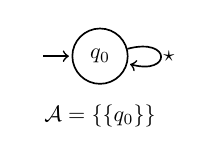
\begin{tikzpicture}[->,shorten >=1pt,auto,node distance=2.8cm,semithick,initial text={},scale=0.8, every node/.style={scale=0.8}]
%
%	
  \node[state,initial] (q0) {$q_0$}; 
  \node[below=1ex of q0] {$\acc = \{ \{ q_0 \} \}$};
%
  \path (q0) edge [loop right]  node[inner sep=1pt] (star) {$\star$} (q0);
\end{tikzpicture}
}
\label{fig:hd-names-omega}
}
%
\hspace{10ex}
\subfigure[]{
{\centering
\begin{tikzpicture}[->,shorten >=1pt,node distance=14ex,auto,semithick,initial text={},scale=0.8, every node/.style={scale=0.8}]
  \tikzstyle{every state}=[minimum size=6ex]
  \tikzstyle{register}=	[circle,fill,draw,inner sep=0pt,minimum size=2pt]	
  \node[state,initial] (q0) {$q_0$}; 
  \node[state,right of=q0] (q1) {};  
  \node (lab1) at (q1) {$q_1$};  \node[register,label={[xshift=-3pt,yshift=-2pt]right:$x$}] (reg) [above=1pt of lab1] {};
	\coordinate (Middle) at ($(q0)!0.5!(q1)$);
  \node[below=4ex of Middle] {$\acc = \{\{q_0,q_1\}\}$};
  \path (q0) edge [bend left]  node[inner sep=1pt] (star) {$\star$} (q1);
  \path (q1) edge[loop right] node[inner sep=1pt] {$\star$} (q1);
  \path (q1) edge [bend left] node {$x$} (q0);
  \path (reg) edge[densely dotted,bend right] (star);
\end{tikzpicture}
}
\label{fig:hd-of-example}
}
%\end{center}
\label{fig:automata}
\vskip -10pt
\caption{Some automata, together with their accepting conditions.
%\subref{fig:example-session} is the nDMA of \cref{exa:session} and \subref{fig:hd-of-example} is the corresponding \hdma; \subref{fig:upwords-ex} is an example \hdma\, where we have omitted the accepting condition and irrelevant transitions, all assumed to end up in a sink state without registers; \subref{fig:hd-names-omega} is the \hdma\ recognizing $\names^\omega$.
}\vskip-10pt
\end{figure}

\noindent Accepted words may fail to be finitely supported. However, languages are. This adheres to the intuition that a machine running forever may read an unbounded amount of different pieces of data, but still have finite memory.
%in line with the intuition of studying machines with finite memory, that never halt.

\begin{theorem}\label{thm:languages-finitely-supported}
 For $\Lang$ a language, and $\pi\in \Perm$, let $\pi\cdot \Lang = \{\pi \cdot \alpha \mid \alpha \in \Lang\}$. For each state $q$ of an nDMA, $\Lang_{q}$ is finitely supported.
\end{theorem}

% \todo{
%  Theorems? First of all, finite support of languages. Also: observation that streams are not finitely supported, but languages are. In the example, what are the finitely supported accepted streams (and how do they differ from the infinitely supported ones?). Can we explain in words the ``finite memory determinacy'' of languages?
% }



\section{Finite automata}\label{sec:hd-automata}
%!TEX root=ndma.tex

In this section, we introduce finite representations of nDMAs. These are similar to classical finite-state automata, but each state is equipped with local registers. There is a notion of assignment to registers, and it is possible to accept, and eventually store, \emph{fresh} symbols. Technically, these structures extend \emph{history-dependent automata} (see \cite{Pistore99}), introducing acceptance of infinite words.

\begin{definition}\label{def:hdma}
 An \emph{history-dependent deterministic Muller automaton} (\hdma) is a tuple $(Q,\weight -,q_0,\rho_0,\htr{}{},\acc)$
 where:
 \begin{itemize}
  \item $Q$ is a finite set of \emph{states};
  \item for $q \in Q$, $\weight{q}$ is a finite set of \emph{local names} (or \emph{registers}) of state $q$;
  \item $q_0 \in Q$ is the \emph{initial state};
  \item $\rho_0 : \weight{q_0} \inj \names$ is the \emph{initial assignment};
  \item $\acc \subseteq \Pow(Q)$ is the \emph{accepting condition}, in the style of \emph{Muller automata};
  \item $\htr{}{}$ is the \emph{transition relation}, made up of quadruples $q_1 \htr{l}{\sigma} q_2$, having \emph{source} $q_1$, \emph{target} $q_2$, label $l \in \weight{q_1} \uplus \{\star\}$, and \emph{history} $\sigma : \weight{q_2} \inj \weight{q_1} \uplus \{l\}$;
  \item the transition relation is \emph{deterministic} in the following sense: for each $q_1 \in Q$,   there is exactly one transition with source $q_1$ and label $\star$, and exactly one transition with source $q_1$ and label $x$ for each $x \in \weight{q_1}$.
 \end{itemize}
\end{definition}
%

\begin{remark}
To keep the notation lightweight, we do not use a \emph{symmetry} attached to states of an \hdma. It is well known (see \cite{MontanariP05}) that symmetries are needed for existence of canonical representatives; we consider this aspect out of the scope of this work. Note that (classical) Muller automata do not have canonical representatives up-to language equivalence. To obtain those, one can use two-sorted structures as in \cite{CV12}. Even though this idea could be applied to hDMAs, this is not straightforward, and requires further investigation.
\label{rem:no-symmetry}
\end{remark}
%
In the following we fix a \hdma{} $A = (Q,\weight -,q_0,\rho_0,\htr{}{},\acc)$. We overload notation (e.g., for the inf-set or the unique run of a word) from \cref{sec:languages}, as it will be always clear from the context whether we are referring to an nDMA or to an \hdma. Acceptance of $\alpha \in \names^\omega$ is defined using the \emph{configuration graph} of $A$.

\begin{definition}\label{def:configuration-graph}
 The set $\confs(A)$ of \emph{configurations} of $A$ consists of the pairs $(q,\rho)$ such that $q \in Q$ and $\rho : \weight q \inj \names$ is an injective \emph{assignment} of names to registers.
\end{definition}

\begin{definition}
\label{def:configuration-graph}
The \emph{configuration graph} of $A$ is a graph with edges of the form  
$(q_1,\rho_1) \tr a (q_2,\rho_2)$ where the source and destination are configurations, and $a \in \names$. There is one such edge if and only if there is a transition $q_1 \htr l \sigma q_2$ in $A$ and either of the following happens: 
 \begin{itemize} 
  \item $l \in \weight{q_1}$, $\rho_1(l) = a$, and $\rho_2 = \rho_1 \circ \sigma$;
  \item $l = \star$, $a \notin \Im(\rho_1)$, $\rho_2 = (\rho_1 \circ \sigma)\sub{a}{\sigma^{-1}(\star)}$.
 \end{itemize}
\end{definition}
% 

The definition deserves some explanation. Fix a configuration $(q_1,\rho_1)$. Say that name $a\in \names$ is \emph{assigned to} the register $x \in \weight{q_1}$ if $\rho_1(x) = a$. When $a$ is not assigned to any register, it is \emph{fresh} for a given configuration. Then the transition $q_1 \htr l \sigma q_2$, under the assignment $\rho_1$, consumes a symbol as follows: either $l \in \weight{q_1}$ and $a$ is the name assigned to register $l$, or $l$ is $\star$ and $a$ is fresh. The destination assignment $\rho_2$ is defined using $\sigma$ as a binding between local registers of $q_2$ and local registers of $q_1$, therefore composing $\sigma$ with $\rho_1$ and eventually adding a freshly received name, whenever $\star$ is in the image of $\sigma$. For readability, we assume that the functional update $\sub{a}{\sigma^{-1}(\star)}$ is void when $\star \notin \Im(\sigma)$. The following lemma clarifies the notion of determinism that we use.

\begin{lemma}
\label{lem:deterministic-configuration-graph}
 For each configuration $(q_1,\rho_1)$ and symbol $a \in \names$, there is exactly one configuration $(q_2,\rho_2)$ such that $(q_1,\rho_1) \tr a (q_2,\rho_2)$.
\end{lemma}
%
We use the notation $(q_1,\rho_1) \Tr{v} (q_2,\rho_2)$ to denote a path that spells $v$ in the the configuration graph. Furthermore, we define runs of infinite words.
%

\begin{definition}
 A \emph{run} $\run$ of an infinite word $\alpha \in \names^\omega$ from configuration $(q,\rho)$ is a sequence $(q_i,\rho_i)$ of configurations, indexed by $\omega$, such that $(q_0,\rho_0)=(q,\rho)$ and for all $i$, in the configuration graph, we have $(q_i,\rho_i) \tr{\alpha_i} (q_{i+1},\rho_{i+1})$. 
\end{definition}

\noindent The following is a simple corollary of  \cref{lem:deterministic-configuration-graph}.

\begin{proposition}
\label{prop:unique-path}
Given $(q_1,\rho_1) \in \confs(A)$ and $v \in \names^\omega$, there exists a unique path $(q_1,\rho_1) \Tr{v} (q_2,\rho_2)$ in the configuration graph of $A$. Similarly, for each word $\alpha$ and configuration $(q,\rho)$, there is a unique run $\run^{\alpha,q,\rho}$ from $(q,\rho)$. We omit $q$ and $\rho$ from the notation, when dealing with the \emph{initial configuration} $(q_0,\rho_0)$.
\end{proposition}

\noindent Finally, we define acceptance of \hdmas. 

\begin{definition}\label{def:acceptance-of-hdmas}
 Consider the unique run $\run$ of an infinite word $\alpha$ from configuration $(q,\rho)$. 
 Let $\Inf(\run)$ denote the set  of states that appear infinitely often in the first component of $\run$. By finiteness of $Q$, $\Inf(\run)$ is not empty. The automaton $A$ accepts $\alpha$ whenever $\Inf(r) \in \acc$. In this case, we speak of the \emph{language} $\Lang_A$ of words accepted by the automaton.
\end{definition}
%
%\begin{figure}[t]
%\centering
%\begin{subfigure}[t]{.4\linewidth}
%\centering
% \begin{tikzpicture}[->,>=stealth',shorten >=1pt,auto,node distance=2.8cm,semithick,initial text={}]
%  %\tikzstyle{every state}=[minimum size=10ex]
%  %\tikzstyle{register}=	[circle,fill,draw,inner sep=0pt,minimum size=2pt]
%	
%  \node[state,initial] (q0) {$q_0$}; 
%  \node[right=10ex of q0] {$\acc = \{ \{q_0 \}\}$ };
%
%  \path (q0) edge [loop right]  node[inner sep=1pt] (star) {$\star$} (q0);
%\end{tikzpicture}
%\subcaption{$\autom_\omega$}
%\[ \acc = \{ \{q_0 \}\} \]
%\label{fig:nomega-hdma}
%\end{subfigure}
%
%\begin{subfigure}[t]{.4\linewidth}
%\centering
% \begin{tikzpicture}[->,>=stealth',shorten >=1pt,node distance=14ex,auto,semithick,initial text={}]
%  \tikzstyle{every state}=[minimum size=6ex]
%  \tikzstyle{register}=	[circle,fill,draw,inner sep=0pt,minimum size=2pt]
%	
%  \node[state,initial] (q0) {$q_0$}; 
%  \node[state,right of=q0] (q1) {};  
%  \node (lab1) at (q1) {$q_1$};
%  \node[register,label={[xshift=-3pt,yshift=-2pt]right:$x$}] (reg) [above=1pt of lab1] {};
%
%
%  \path (q0) edge [bend left]  node[inner sep=1pt] (star) {$\star$} (q1);
%  \path (q1) edge[loop right] node[inner sep=1pt] {$\star$} (q1);
%  \path (q1) edge [bend left] node {$x$} (q0);
%  \path (reg) edge[densely dashed,bend right] (star);
%\end{tikzpicture}
%\[\acc = \{ \{ q_0,q_1 \} \}\]
%\subcaption{$\autom_{s}$}
%\label{ex:session-hdma}
%\end{subfigure}
%
%\caption{Example \hdmas: labelled dots within states represent registers, dashed lines depict the action of history maps.}
%\label{fig:ex-hdmas}
%\end{figure}
%
%
%
As an example, the language $\names^\omega$ of all infinite words over $\names$ is recognised by the \hdma\ %having one state $q$, with $\weight q = \emptyset$ and one transition from $q$ to $q$, labelled by $\star$ (see 
in \cref{fig:hd-names-omega}; the initial assignment $\rho_0$ is necessarily empty, and so is the history $\sigma$ along the transition.
%
%
Differently from nDMAs, \hdmas\ have finite states. 
%\todo{La frase The configuratoin graph... infinite-branching a che serve? La togliamo?} The configuration graph is deterministic, even if still infinite-state and infinite-branching.
Finite representations are useful for effective operations on languages, as we shall see later. The similarity between configuration graphs of \hdmas, and nDMAs, is deep, as stated in the following propositions. These are similar to the categorical equivalence results in \cite{GadducciMM06,FioreS06}; however, notice that representing infinite branching systems using  ``allocating transitions'' requires further machinery, similar to what is studied in \cite{CianciaM10}. See also \cref{rem:no-symmetry} about symmetry.

\begin{figure}[t]
\centering
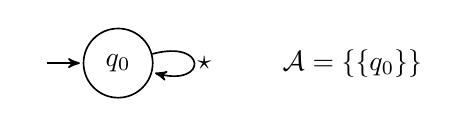
\begin{tikzpicture}[->,>=stealth',shorten >=1pt,auto,node distance=2.8cm,semithick,initial text={}]
  %\tikzstyle{every state}=[minimum size=10ex]
  %\tikzstyle{register}=	[circle,fill,draw,inner sep=0pt,minimum size=2pt]
	
  \node[state,initial] (q0) {$q_0$}; 
  \node[right=10ex of q0] {$\acc = \{ \{q_0 \}\}$ };

  \path (q0) edge [loop right]  node[inner sep=1pt] (star) {$\star$} (q0);
\end{tikzpicture}
\caption{The \hdma{} accepting $\names^\omega$.}
\label{fig:hd-names-omega}
\end{figure}

\begin{proposition}\label{pro:nset-to-nom}
 The configuration graph of $A$, equipped with the permutation action $\pi \cdot (q,\rho) = (q,\pi \circ \rho)$ forms the transition structure of an nDMA. The orbits of the obtained nDMA are in one to one correspondence with states in $Q$; thus the acceptance condition on states can be used as an acceptance condition on the orbits of the configuration graph. When the configuration $(q_0,\rho_0)$ is chosen as initial state, the obtained nDMA accepts the same language as $A$.
\end{proposition}
%
%\noindent It is also possible to obtain an equivalent hDMA from a nDMA.
%See the proof of the next proposition for details on the construction.

\begin{proposition}\label{prop:ndma-to-hdma}
For each nDMA $(Q,\tr{},q_0,\acc)$, there is an \hdma{} accepting the same language.
For $q \in Q$ , let $o_q$ be a chosen canonical representative of $\orb(q)$, $o_{S \subseteq X} = \{o_q \mid q \in S\}$ and $\rho_q$ be a chosen permutation such that $\rho_q \cdot o_q = q$.	Construct the \hdma\  $(o_Q,\weight-,\htr{}{},o_{q_0},\restr{\rho_{q_0}}{\weight{o_{q_0}}},\{ \{ o_q \mid q \in A\} \mid A \in \acc \})$, 
%
with $\weight{o_q} = \supp(o_q)$. For each nDMA transition $o_{q_1} \tr a o_{q_2}$, if $a \in \supp(o_{q_1})$, let $o_{q_1} \htr{a}{\sigma} o_{q_2}$; otherwise, let $o_{q_1} \htr{\star}{\sigma_\star} o_{q_2}$, where $\sigma=\restr{\rho_{q_2}}{\weight{o_{q_2}}}$ and $\sigma_\star = \restr{\sigma_{q_2}\sub{*}{a}}{\weight{o_{q_2}}}$.
\end{proposition}


\begin{example}
Consider the following \hdma{} 

\begin{center}
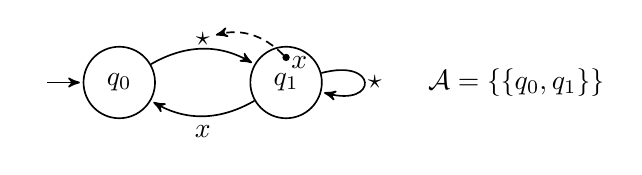
\begin{tikzpicture}[->,>=stealth',shorten >=1pt,node distance=14ex,auto,semithick,initial text={}]
  \tikzstyle{every state}=[minimum size=6ex]
  \tikzstyle{register}=	[circle,fill,draw,inner sep=0pt,minimum size=2pt]
	
  \node[state,initial] (q0) {$q_0$}; 
  \node[state,right of=q0] (q1) {};  
  \node (lab1) at (q1) {$q_1$};
  \node[register,label={[xshift=-3pt,yshift=-2pt]right:$x$}] (reg) [above=1pt of lab1] {};
  \node[right=8ex of q1] {$\acc = \{\{q_0,q_1\}\}$};

  \path (q0) edge [bend left]  node[inner sep=1pt] (star) {$\star$} (q1);
  \path (q1) edge[loop right] node[inner sep=1pt] {$\star$} (q1);
  \path (q1) edge [bend left] node {$x$} (q0);
  \path (reg) edge[densely dashed,bend right] (star);
\end{tikzpicture}
\end{center}
%
where the labelled dot within $q_1$ represents its register, and the dashed line depicts the history from $q_1$ to $q_0$ (we omit empty histories). This automaton accepts the language of \cref{exa:session}. In fact, $q_0$ is the only element in the orbit of the initial state of the nDMA, and $q_1$ canonically represents all $q_a$, $a \in \names$. This notation for \hdmas{} will be used throughout the paper.\end{example}



% 
% \begin{definition}
%  The configuration graph of $A$ consists of the set of configurations equipped with a ternary transition relation, labelled with names. Specifically, we have $(q_1,\rho_1) \tr a (q_2,\rho_2)$, with $a \in \names$ if and only if 
% \end{definition}



\section{Ultimately-periodic words}\label{sec:up-words}%!TEX root=ndma.tex
%
%

\begin{figure}[t]
\begin{center}
 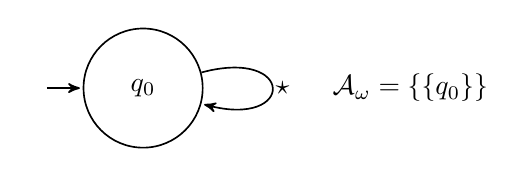
\begin{tikzpicture}[->,>=stealth',shorten >=1pt,auto,node distance=2.8cm,semithick,initial text={}]
  \tikzstyle{every state}=[minimum size=10ex]
  \tikzstyle{register}=	[circle,fill,draw,inner sep=0pt,minimum size=2pt]
	
  \node[state,initial] (q0) {$q_0$}; 
  \node[right=10ex of q0] {$\acc_\omega = \{ \{q_0 \}\}$ };

  \path (q0) edge [loop right]  node[inner sep=1pt] (star) {$\star$} (q0);
\end{tikzpicture}

\end{center}
\caption{Automaton $\autom_\omega$ for $\names^\omega$.}
\label{fig:nomega-automaton}
\end{figure}

\begin{figure}[t]
\begin{center}
 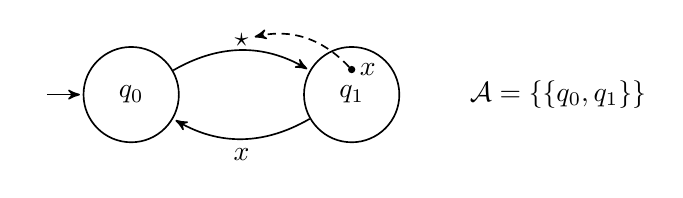
\begin{tikzpicture}[->,>=stealth',shorten >=1pt,auto,node distance=2.8cm,semithick,initial text={}]
  \tikzstyle{every state}=[minimum size=8ex]
  \tikzstyle{register}=	[circle,fill,draw,inner sep=0pt,minimum size=2pt]
	
  \node[state,initial] (q0) {$q_0$}; 
  \node[state,right of=q0] (q1) {};  
  \node (lab1) at (q1) {$q_1$};
  \node[register,label={[xshift=-2pt]right:$x$}] (reg) [above=1pt of lab1] {};
  \node [right=5ex of q1] {$\acc = \{ \{ q_0,q_1 \} \}$};


  \path (q0) edge [bend left]  node[inner sep=1pt] (star) {$\star$} (q1);
  \path (q1) edge [bend left] node {$x$} (q0);
  \path (reg) edge[densely dashed,bend right] (star);
\end{tikzpicture}
\end{center}
\caption{\label{fig:upwords} Automaton for the language of \cref{exa:session}.}
\end{figure}

\tbox{Sezione 4?}
{
Given a sequence $P$ of transitions in $A$, we write $(q_1,\rho_1) \TrP{v}{P} (q_2,\rho_2)$ whenever $(q_1,\rho_1) \Tr{v} (q_2,\rho_2)$ and such path is induced by $P$.
}
%
An \emph{ultimately periodic} word is a word of the form $uv^\omega$, with $u,v$ finite words. Given a $\omega$-regular language $\Lang$, let $UP(\Lang)$ be its ultimately periodic fragment, namely $\{ \alpha \in \Lang \mid \alpha = uv^\omega \land u,v \; \text{are finite} \}$. Then, for every two languages $\Lang_1$ and $\Lang_2$, $UP(\Lang_1) = UP(\Lang_2)$ implies $\Lang_1 = \Lang_2$ \cite{CalbrixNP93}, in words: $\omega$-regular languages are characterized by their ultimately periodic fragments.

In this section we aim to extend this result to the nominal setting. The preliminary result to establish, as in the classical case, is that every non-empty $\omega$-regular nominal language $\Lang$ contains at least one ultimately periodic word. For $\omega$-regular languages, this involves finding a loop through accepting states in the automaton and iterating it. In our case this is not enough, because it may not be possible to consume the same name in consecutive traversals of the same transition due to freshness. The first part of this section will be spent in showing that, given a loop in a \hdma{}, there always is a path induced by consecutive traversals of the loop, such that its initial and final configurations coincide. This implies that such path can be taken an arbitrary number of times.

We fix a loop (the specific \hdma{} is not relevant)
\[
	L \;:=\; p_0 \htr{l_0}{\sigma_0} p_1 \htr{l_1}{\sigma_1} \dots \htr{l_{n-1}}{\sigma_{n-1}} p_0
\]
We write $\ul{i}$ for $i \mod n$. Let $\widehat{\sigma}_i \colon \weight{p_\ul{i+1}} \pto \weight{p_i}$ be the partial maps telling the history of old registers and ignoring the new ones, formally
\[
	\widehat{\sigma}_i := \sigma_i \setminus \{ (x,y) \in \sigma_i \mid y = \star \} 
	\qquad (i=0,\dots,n-1)
\]
and let $\widehat{\sigma} \colon \weight{p_0} \pto \weight{p_0}$ be their composition $\widehat{\sigma}_0 \circ \widehat{\sigma}_1 \dots \circ \widehat{\sigma}_{n-1}$. We define the set $I$ as the greatest subset of $\dom(\widehat{\sigma})$ such that $ \widehat{\sigma}(I) = I$,
i.e.\ $I$ are the registers of $p_0$ that ``survive'' along $L$. We denote by $T$ all the other registers, namely $T := \weight{p_0} \setminus I$. These are registers whose content is eventually discarded (not necessarily within a single loop traversal), as the following lemma states.
%
%
\begin{lemma}
\label{lem:rho-forget}
Given any $x \in T$, let $\{x_j\}_{j \in J_x}$ be the smallest sequence that satisfies the following conditions:
$
	x_0 = x
$
and
$
	x_{j+1} = \sigma_{\ul{j}}^{-1}(x_j),
$
where $j+1 \in J_x$ only if $\sigma_{\ul{j}}^{-1}(x_i)$ is defined. Then $J_x$ has finite cardinality.
\end{lemma}
%
Now, consider any assignment $\rrho_0 \colon \weight{p_0} \to \names$. We give some lemmata about paths that start from $(p_0,\rrho_0)$ and are induced by consecutive traversals of $L$. The first one says that the assignment for $I$ given by $\rrho_0$ is always recovered after a fixed number of traversals of $L$, regardless of which symbols are consumed.
%
\begin{lemma} 
\label{lem:idI}
There is $\id \geq 1$ such that, for all $v_0,\dots,v_{\id-1}$ satisfying
\[
	(p_0,\rrho_0) \TrP{v_0}{L} (p_0,\rrho_1) \TrP{v_1}{L} \dots \TrP{v_{\id-1}}{L} (p_0,\rrho_\id)
\]
we have $\restr{ \rrho_\id }{I} = \restr{ \rrho_0 }{I}$.
\end{lemma}
%
The second one says that, after a minimum number of traversals of $L$, a configuration can be reached where the initial values of $T$, namely those assigned by $\rrho_0$, cannot be found in any of the registers.
%
\begin{lemma}
There is $\forg \geq 1$ such that, for all $\gamma \geq \forg$ ,there are $v_0,\dots,v_{\gamma-1}$ satisfying
\[
	(p_0,\rrho_0) \TrP{v_0}{L} (p_0,\rrho_1) \TrP{v_1}{L} \dots \TrP{v_{\gamma-1}}{L} (p_0,\rrho_\gamma)
	\qquad 
	\Im(\rrho_\gamma) \cap \rrho_0(T) = \varnothing \enspace .
\]
\label{lem:forgetT}
\end{lemma}
%
%
Finally, we give the dual of the previous lemma: if we start from a configuration where registers are not assigned values in $\rrho_0(T)$, then these values can be assigned back to $T$ in a fixed number of traversals of $L$, regardless of the initial assignment.

\begin{lemma}
There is $\ass \geq 1$ such that,
for any $\trho_0 \colon \weight{p_0} \to \names$ with $\Im(\trho_0) \cap \rrho_0(T) = \varnothing$, there are $v_0,\dots,v_{\ass-1}$ satisfying
\[
	(p_0,\trho_0) \TrP{v_0}{L} (p_0,\trho_1) \TrP{v_1}{L} \dots \TrP{v_{\ass-1}}{L} (p_0,\trho_\ass)	
	\qquad
	\restr{\trho_\ass}{T} = \restr{\rrho_0}{T} \enspace .
\]
\label{lem:initT}
\end{lemma}
%
\vspace{-4ex}
%
Finally, we combine the above lemmata. We construct a path where: (1) the values assigned to $T$ are forgotten and then recovered (2) the values assigned to $I$ are swapped, but the initial assignment is periodically regained. Therefore, the length of such path should allow (1) and (2) to ``synchronize'', so that the final assignment is again $\rrho_0$.

\begin{theorem}
\label{thm:loop}


There are $v_0,\dots,v_n$ such that
\[
	(p_0, \rrho_0) \TrP{v_0}{L} (p_0, \rrho_1) \TrP{v_1}{L} \cdots \TrP{v_n}{L} (p_0,\rrho_0) \enspace .
\]
\end{theorem}

\begin{proof}
We can take any path of the form
\[
	(p_0,\rrho_0) \TrP{v_0}{L} (p_0,\rrho_1) \TrP{v_1}{L} \cdots \TrP{v_{\gamma-1}}{L} (p_0,\rrho_\gamma) \TrP{v_{\gamma}}{L} \cdots \TrP{v_{\gamma + \ass - 1}}{L} (p_0,\rrho_{\gamma + 
	 \ass})
\]
where the part from $(p_0,\rrho_0)$ to $(p_0,\rrho_\gamma)$ is given by \cref{lem:forgetT} and the remaining subpath is given by \cref{lem:initT}, with $\trho_0 = \rrho_\gamma$. The only constraint about $\gamma$ is that there should be a positive integer $\lambda$ such that $\gamma + \ass = \lambda \id$, where $\id$ is given by \cref{lem:idI}. The claim follows from $\restr{\rrho_{\gamma + \ass}}{T} = \restr{\rrho_0}{T}$ and 
$\restr{\rrho_{\gamma + \ass}}{I} = \restr{\rrho_0}{I}$ which, together with $I \cup T = \weight{p_0}$, imply $\rrho_{\gamma + \ass} = \rrho_0$.
\qed
\end{proof}
%

\begin{figure}[t]
\begin{center}
 \begin{tikzpicture}[->,>=stealth',shorten >=1pt,auto,node distance=2.8cm,semithick,initial text={}]
  \tikzstyle{every state}=[minimum size=10ex]
  \tikzstyle{register}=	[circle,fill,draw,inner sep=0pt,minimum size=2pt]
	
  \node[register,label={[shift={(2pt,-2pt)}]above:$x_0$}] (reg00) {};
  \node[register,label={[shift={(2pt,-2pt)}]above:$y_0$}] (reg01) [right=10pt of reg00] {};
  \node[register,label={[shift={(2pt,-2pt)}]above:$z_0$}] (reg02) [right=10pt of reg01] {};

  \node[register,label={[shift={(2pt,-2pt)}]above:$x_1$}] (reg10) [right=50pt of reg02] {};
  \node[register,label={[shift={(2pt,-2pt)}]above:$y_1$}] (reg11) [right=10pt of reg10] {};
  \node[register,label={[shift={(2pt,-2pt)}]above:$z_1$}] (reg12) [right=10pt of reg11] {};

  \node[register,label={[shift={(2pt,-2pt)}]above:$y_2$}] (reg21) at ($(reg02)!0.5!(reg10)$) [yshift=-15ex] {};

  \node[register,label={[shift={(2pt,-2pt)}]above:$x_2$}] (reg20) [left=10pt of reg21] {};
  \node[register,label={[shift={(2pt,-2pt)}]above:$z_2$}] (reg22) [right=10pt of reg21] {};



  \node[state,initial,fit={(reg00) (reg01) (reg02)},inner sep=2ex] (q0) {};
  \node[above left=-1ex of q0] (lab0) {$q_0$}; 
  \node[state,fit={(reg10) (reg11) (reg12)},inner sep=2ex] (q1) {};
  \node[above right=-1ex of q1] (lab1) {$q_1$}; 
  \node[state,fit={(reg20) (reg21) (reg22)},inner sep=2ex] (q2) {};
  \node[below=1pt of q2] (lab2) {$q_2$}; 

  \path (q0) edge [bend left] node {$z_0$} (q1);
  \path (q1) edge [bend left]  node[inner sep=1pt] (star) {$\star$} (q2);
  \path (q2) edge [bend left] node {$x_2$} (q0);
	
  \path (reg10) edge[densely dashed,out=90,in=90,looseness=2,shorten >=7pt,shorten <=8pt] (reg01);
  \path (reg11) edge[densely dashed,out=90,in=90,looseness=2,shorten >=7pt,shorten <=8pt] (reg00);
  \path (reg12) edge[densely dashed,out=90,in=90,looseness=2,shorten >=7pt,shorten <=8pt] (reg02);

  \path (reg20) edge[densely dashed,shorten <=8pt] (reg10);
  \path (reg21) edge[densely dashed,shorten <=8pt] (reg11);
  \path (reg22) edge[bend right,densely dashed] (star);

  \path (reg20) edge[densely dashed,shorten <=5pt] (reg00);
  \path (reg21) edge[densely dashed,shorten <=5pt] (reg01);
  \path (reg22) edge[densely dashed,shorten <=5pt] (reg02);

\end{tikzpicture}

\end{center}
\caption{\label{fig:upwords-ex} An example automaton. Some transitions are not shown: they are all assumed to end up in a sink state without registers.}
\end{figure}

\begin{example} We justify the above construction on the automaton in \cref{fig:upwords-ex}, with initial assignment $\rho_0(x_0) = a$,$\rho_0(y_0) = b$ and $\rho_0(z_0) = c$. We omit the accepting set, as it is not relevant. Consider the loop $L$ formed by all the depicted transitions.
We have $I = \{x_0,y_0\}$ and $T = \{z_0\}$. Consider the path
\begin{align*}
	(q_0,[\subs{a}{x_0},\subs{b}{y_0},\subs{c}{z_0}]) \tr{c} (q_1,[\subs{b}{x_1},\subs{a}{y_1},\subs{c}{z_1}]) &\tr{d} (q_2,[\subs{b}{x_2},\subs{a}{y_2},\subs{d}{z_2}]) \\
	&\tr{b} (q_0,[\subs{b}{x_0},\subs{a}{y_0},\subs{d}{z_0}])
\end{align*}
where $d \neq a,b,c$. Notice that the values of $x_0$ and $y_0$ get swapped according to the permutation $(a \; b)$, and $d$ is assigned to $z_0$. Our aim is to recover $\rho_0$ again. According to \cref{lem:idI}, $x_0$ and $y_0$ get their assignment back in $\theta = 2$ traversals of $L$ (in fact $(a\; b)^2 = (a\; b)$). As for $z_0$, its assignment is established in the second transition, but $c$ should not have been assigned to any register of $q_1$ in order for it to be consumed during this transition. This is where \cref{lem:forgetT} comes into play: it says that in at least $\epsilon = 1$ traversals of $L$ the name $c$ is discarded. This is exactly what happens in the path shown above. Then we can assign $c$ to $z_0$ in another $\zeta = 1$ traversal of $L$, according to \cref{lem:initT}. Since $\epsilon + \zeta  = \theta = 2$, traversing $L$ twice is enough. For instance, we can take the path spelling $cdbdca$.
\end{example}


Finally we have the main results.
%
\begin{theorem}
\label{thm:up-fragment}
Every non-empty $\omega$-regular nominal language $\Lang$ has an ultimately periodic fragment.
\end{theorem}
\begin{proof}
Let $\autom$ be the automaton for $\Lang$. Take any $\alpha \in \Lang$ and let $I = \Inf(r^\alpha)$ (recall $r^\alpha$ is the run for $\alpha$ in $\autom$), so $I \in \acc$. A path spelling $\alpha$ in the configuration graph of $A$ must \todo{Spiegare meglio perchè ``must''?} begin with
\[
	(q_0,\rho_0) \Tr{u} (q_1,\rho_1) \TrP{v}{P} (q_1,\rho_2)
\]
where $q_1 \in I$ and $(q_1,\rho_1) \TrP{v}{P} (q_2,\rho_2)$ is such that $P$ goes through all the states in $I$. Since $P$ is a loop, we can replace its induced path with a new one given by \cref{thm:loop} 
\[
	(q_0,\rho_0) \Tr{u} (q_1,\rho_1) \TrP{v_0}{P} \cdots \TrP{v_n}{P} (q_1,\rho_1) \enspace .
\]
This subpath can be traversed any number of times, so we have $u(v_0\dots v_n)^\omega \in \Lang$.
\qed
\end{proof}

\begin{theorem}
Let $\Lang_1,\Lang_2$ be $\omega$-regular nominal languages. Then $UP(\Lang_1) = UP(\Lang_2)$ implies $\Lang_1 = \Lang_2$.
\end{theorem}
\begin{proof}
Consider the language $(\Lang_1 \cup \Lang_2) \setminus (\Lang_2 \cap \Lang_2)$. By \cref{thm:bool-closure}, this is a $\omega$-regular nominal language. Suppose it is not empty, i.e.\ $\Lang_1 \neq \Lang_2$. Then, by \cref{thm:up-fragment}, it must contain at least one ultimately periodic word, so also $UP(\Lang_1) \neq UP(\Lang_2)$, a contradiction.
\end{proof}


\section{Synchronized product}\label{sec:sync-product}
%!TEX root=ndma.tex
\newcommand{\eq}[1]{#1}
\newcommand{\syncQ}{Q_{\syncp}}
\newcommand{\syncW}[1]{\weight{#1}_{\syncp}}
\newcommand{\syncAss}{\rho_0^{\syncp}}
\newcommand{\syncInit}{q_0^{\syncp}}
\newcommand{\syncTr}[1]{\xymatrix@C-=4ex{\ar[r]^{#1}&\!_{\syncp}}}
\newcommand{\syncHtr}[2]{\xymatrix@C-=4ex{\ar[r]^{#1}_{#2}&\!_{\syncp}}}
\newcommand{\regrule}{\textsc{(Reg)}}
\newcommand{\allrule}{\textsc{(Alloc)}}
\newcommand{\cproj}{\pi}

The product of two finite automata uses the well-known \emph{synchronised product} construction. In this section we define this operation on the underlying \emph{transition structures} of \hdmas{}, i.e.\ on tuples $\tstr = (Q,\weight{-},q_0,\rho_0,\trarrow)$ (we want to be parametric w.r.t.\ the accepting condition). One should  be careful in handling registers. When forming pairs of states, some of these registers could be constrained to have the same value.
%assignments are injective. 
Thus, states have the form $(q_1,q_2,R)$, where $R$ is a relation, linking registers of $q_1$ and $q_2$, that represent the same register in the synchronised product. This is implemented by quotienting registers w.r.t.\ the equivalence $R^*$ induced by $R$; the construction is similar to the case of register automata, and to the construction of products in named sets given in \cite{CianciaM10}.

Given two transition structures $\tstr_i = (Q_i,\weight{-}_i,q_0^i,\rho_0^i,\trarrow_i)$, $i=1,2$, we define their synchronized product $\tstr_1 \syncp \tstr_2$. Given $q_1 \in Q_1$,$q_2 \in Q_2$, $Reg(q_1,q_2)$ is the set of relations that are allowed to appear in states of the form $(q_1,q_2,R)$, namely those $R \subseteq \weight{q_1}_1 \times \weight{q_2}_2$ such that, for each $(x,y) \in R$, there is no other $(x',y') \in R$ with $x'=x$ or $y'=y$. This avoids inconsistent states where the individual assignment for $q_1$ or $q_2$ would not be injective. In the following we assume $[x]_{R^*}$ (the canonical representative of the equivalence class of $x$ in $R^*$) to be $\{x\}$ when $x$ does not appear in any pair of $R$.

% These relations, when appearing within states of $\tstr_1 \syncp \tstr_2$, avoid two register of the same state to be assigned the same value.

% to be paired with the same of $q_2$ or viceversa, because this would mean that $x_1$ and $x_2$ should be assigned the same value, but assignments are injective. We assume that $R$ is implicitly 

%that we allow to appear in states of $\tstr_1 \syncp \tstr_2$ where $q_1$ and $q_2$ are paired
%\[
%	Reg(q_1,q_2) := \{ R \subseteq \weight{q_1}_1 \times \weight{q_2}_2 \mid (x_1,y_1),(x_2,y_2) \in R \implies x_1 \neq x_2 \land y_1 \neq y_2 \}
%\]
%We avoid relations where two (or more) registers $x_1,x_2$ of $q_1$ are paired with the same one of $q_2$ or viceversa, because this would mean that $x_1$ and $x_2$ should be assigned the same value, but assignments are injective. Notice that $R \in Reg(q_1,q_2)$ is such that equivalence classes of $R^*$ have cardinality at most two.


\begin{definition}
\label{def:syncp}
$\tstr_1 \syncp \tstr_2$ is the tuple $(\syncQ,\syncW{-},\syncInit,\syncAss,\syncTr{\quad})$ where:
\begin{itemize}
	\item 
	%$\syncQ := \bigcup_{q_1 \in Q_1,q_2 \in Q_2} \{(q_1,q_2)\} \times Reg(q_1,q_2)$;
	$\syncQ := \{ (q_1,q_2,R) \mid q_1 \in Q_1,q_2 \in Q_2,R \in Reg(q_1,q_2)\}$;
	%
	\item $\syncW{(q_1,q_2,R)} := (\weight{q_1}_1 \cup \weight{q_2}_2)_{/R^*}$, for $(q_1,q_2,R) \in \syncQ$;
	%
	\item $\syncInit := (q_0^1,q_0^2,R_0)$, where $R_0:= \{ (x_1,x_2) \in \weight{q_0^1}_1 \times \weight{q_0^2}_2 \mid \rho_0^1(x_1) = \rho_0^2(x_2) \}$;
	%
	\item $\rho_0([x]_{R_0^*}) = \rho_0^i (x)$ whenever $x \in \weight{q_0^i}_i$, $i \in \{1,2\}$; 
	%
	\item transitions are generated by the following rules
\end{itemize}
	%
		\begin{mathpar}
			\inferrule[(Reg)]
			{ q_1 \htrind{l_1}{\sigma_1}{1} q_1' \\
			q_2 \htrind{l_2}{\sigma_2}{2} q_2' 
			\\\\
			\exists i \in \{1,2\} : l_i \in \names \land [l_i]_{R^*} = \{l_1,l_2\} \cap \names}
			%\cap \names \quad i \in \{1,2\}}
			{ (q_1,q_2,R) \syncHtr{[l_i]_{R^*}}{\sigma_R}
			(q_1',q_2',S) } 
			%}
			\quad\;
			\inferrule[(Alloc)]
			{ q_1 \htrind{l_1}{\sigma_1}{1} q_1' \quad q_2 \htrind{l_2}{\sigma_2}{2} q_2' \quad l_1,l_2 = \star} 
			{ (q_1,q_2,R) \syncHtr{\star}{\sigma_A} (q_1',q_2',S) }
		\end{mathpar}
	%\vspace{-2ex}
	where $S := \sigma_2^{-1} \circ R \cup \{(l_1,l_2)\} \circ \sigma_1 $ and
% and the mappings $\sigma_\tau$, for $\tau \in \{A,R\}$, are as follows
	\begin{align*}
		%S &:= \sigma_2^{-1} \circ R \cup \{(l_1,l_2)\} \circ \sigma_1 
		%\\[2ex]
		\sigma_\tau([x]_{S^*}) &:= 
		\begin{cases}
			[\sigma_i(x)]_{R^*} & x \in \weight{q'_i}_i \land \sigma_i(x) \neq \star \\
			[l_{3-i}]_{R^*} & x \in \weight{q'_i}_i \land \sigma_i(x) = \star \land \tau = R \\
			\star & x \in \weight{q'_i}_i \land \sigma_i(x) = \star \land \tau = A
		\end{cases}
	\end{align*}
%\end{itemize}
\end{definition}
%
 Before explaining in detail the formal definition, we remark that the relation $S$ is well defined, i.e.\ it belongs to $Reg(q_1',q_2')$: the addition of $\{(l_1,l_2)\}$ to $R$ is harmless, as will be explained in the following, and $\sigma_1$ and $\sigma^{-1}_2$ can never map the same value to two different values (as they are functions) or vice versa (as they are injective).
%
The definition of $\syncInit$ motivates the presence of relations in states: $R_0$-related registers are the ones that are assigned the same value by $\rho_0^1$ and $\rho_0^2$; these form the same register of $\syncInit$, so $\syncAss$ is well-defined. The synchronization mechanism is implemented by rules \regrule{} and \allrule{}: they compute transitions of $(q_1,q_2,R) \in \syncQ$ from those of $q_1$ and $q_2$ as follows.

Rule \regrule{} handles two cases. First, if the transitions of $q_1$ and $q_2$ are both labelled by registers, say $l_1$ and $l_2$, and these registers correspond to the same one in $(q_1,q_2,R)$ (condition $[l_i]_{R^*} = \{l_1,l_2\}$, recalling that $[l_i]_{R^*}$ cannot contain more labels due to injectivity of register maps), then \regrule{} infers a transition labelled with $[l_i]_{R^*}$ (the specific $i$ is not relevant). The target state of this transition is made of those of the transitions from $q_1$ and $q_2$, plus a relation $S$ obtained by translating $R$-related registers to $S$-related registers via $\sigma_1$ and $\sigma_2$. In this case, adding the pair $(l_1,l_2)$ to $R$ in the definition of $S$ has no effect, as it is already in $R$. The inferred history $\sigma_R$ just combines $\sigma_1$ and $\sigma_2$, consistently with $S^*$.

The other case for \regrule{} is when a fresh name is consumed from just one state, e.g.\ $q_2$.
This name must coincide with the value assigned to the register $l_1$ labelling the transition of $q_1$. Therefore the inferred label is $[l_1]_{R^*}$. The target relation $S$ changes slightly. Suppose there are $l'_1 \in \weight{q'_1}$ and $l'_2\in \weight{q'_2}$ such that $\sigma_1(l'_1) = l_1$ and $\sigma_2(l'_2) = \star$; after $q_1$ and $q_2$ perform their transitions, both these registers are assigned the same value, so we require $(l'_1,l'_2) \in S$. This pair is forced to be in $S$ by adding $(l_1,\star)$ to $R$ when computing $S$. This does not harm well-definedness of $S$, because $[l_1]_{R^*}$ is a singleton (rule premise $[l_1]_{R^*} = \{l_1,\star\} \cap 	\names = \{l_1\}$), so no additional, inconsistent identifications are added to $S^*$ due to transitivity. If either $l_1$ or $\star$ is not in the image of the corresponding history map, then augmenting $R$ has no effect, as the relational composition discards $(l_1,\star)$. The history $\sigma_R$ should map $[l_2']_{S^*}$ to $[l_1]_{R^*}$: this is treated by the second case of its definition; all the other values are mapped as before.

Transitions of $q_1$ and $q_2$ consuming a fresh name on both sides are turned by \allrule{} into a unique transition with freshness: $S$ is computed by adding $(\star,\star)$ to $R$, thus the registers to which the fresh name is assigned (if any) form one register in the overall state; the inferred history $\sigma_A$ gives the freshness status to this register, and acts as usual on other registers.

\begin{remark}
\label{rem:syncp-fin-det}
$\tstr_1 \syncp \tstr_2$ is finite-state and deterministic. In fact, every set in the definition of $\syncQ$ is finite.
%, and cartesian products, powerset and finite union of finite sets again yield finite sets.
As for determinism, given $(q_1,q_2,R) \in \syncQ$, each $l \in \syncW{(q_1,q_2,R)} \cup \{\star\}$ uniquely determines which labels $l_1$ and $l_2$ should appear in the rule premises (e.g. if $l = \{l_1\}$, with $l_1 \in \weight{q_1}_1$, then $l_2 = \star$), and by determinism each $q_i$ can do a unique transition labeled by $l_i$.
\end{remark}
%
We shall now relate the configuration graphs of $\tstr_1 \syncp \tstr_2$, $\tstr_1$ and $\tstr_2$.
%
\begin{definition}
Let $((q_1,q_2,R),\rho) \in \confs(\tstr_1 \syncp \tstr_2)$. Its $i$-th projection, denoted $\cproj_i$, is defined as
$\cproj_i((q_1,q_2,R),\rho) = (q_i,\rho_i)$ with $\rho_i := \lambda x \in \weight{q_i}_i.\rho([x]_{R^*})$
\end{definition}
%
Projections always produce valid configurations in $\confs(\tstr_1)$ and $\confs(\tstr_2)$: injectivity of $\rho_i$ follows from the definition of $Reg(q_1,q_2)$, ensuring that two different $x_1,x_2 \in \weight{q_i}_i$ cannot belong to the same equivalence class of $R^*$, i.e.\ cannot have the same image through $\rho_i$. The correspondence between edges is formalized as follows.

\begin{proposition}
%\todo{condensare, usando $\pi_i$ invece di $\pi_1,\pi_2$?}
\label{prop:edges-correspondence}
Given $C \in \confs(\tstr_1 \syncp \tstr_2)$: 
\begin{inparaenum}[(i)]
	\item %\vskip -6pt 
	if $C \tr{a} C'$ then $\cproj_i(C) \tr{a} \cproj_i(C')$, $i = 1,2$;
	% and $\cproj_2(C) \tr{a} \cproj_2(C')$;
	\label{sync-to-each}
	\item if $\cproj_i(C) \trind{a}{i} C_i$, $i=1,2$, 
	%and $\cproj_2(C) \trind{a}{1} C_2$, 
	then $\exists C' : C\tr{a} C'$ and $\cproj_i(C) = C_i$.
	%,$\cproj_2(C) = C_2$.
	\label{each-to-sync}
\end{inparaenum}
% \begin{enumerate}[(i)]
% 	\item if $C \tr{a} C'$ then $\cproj_i(C) \tr{a} \cproj_i(C')$, $i = 1,2$;
% 	% and $\cproj_2(C) \tr{a} \cproj_2(C')$;
% 	\label{sync-to-each}
% 	\item if $\cproj_i(C) \trind{a}{i} C_i$, $i=1,2$, 
% 	%and $\cproj_2(C) \trind{a}{1} C_2$, 
% 	then there is $C'$ s.t.\ $C\tr{a} C'$ and $\cproj_i(C) = C_i$.
% 	%,$\cproj_2(C) = C_2$.
% 	\label{each-to-sync}
% \end{enumerate}
\end{proposition}
%
\begin{corollary}
\label{cor:paths-correspondence}
Let $C_0 = (\syncInit,\rho_0)$. We have a path $C_0 \tr{a_0} \dots \tr{a_{n-1}} C_n$ in the configuration graph of $\tstr_1 \syncp \tstr_2$ if and only if we have paths $\cproj_i(C_0) \tr{a_0} \dots \tr{a_{n-1}} \cproj_i(C_n)$ in the configuration graphs of $\tstr_i$, for $i=1,2$. The correspondence clearly holds also for infinite paths, i.e.\ runs.
\end{corollary}
%
This result allows us to relate the $\Inf$ of runs in the defined transition structures.%\todo{check sentence}
%
\begin{theorem}
\label{thm:inf-correspondence}
Given $\alpha \in \names^\omega$, let $r$ be a run for $\alpha$ in the configuration graph of $\tstr_1 \syncp \tstr_2$, and let $r_1$ and $r_2$ be the corresponding 
%\todo{Non capisco: paths o runs? Estenderei il corollario per parlare di runs, se è banale} 
runs for $\tstr_1$ and $\tstr_2$, according to \cref{cor:paths-correspondence}. Then $\pi_1(Inf(r)) = Inf(r_1)$ and $\pi_2(Inf(r)) = Inf(r_2)$.
\end{theorem}

\section{Boolean operations and decidability}\label{sec:boolean-operations-decidability}%!TEX root=ndma.tex
\newcommand{\compl}[1]{\overline{#1}}
 
In this section we discuss closure of $\omega$-regular nominal languages under boolean operations, and decidability of emptiness and language equality.

Let $\Lang_1$ and $\Lang_2$ be $\omega$-regular nominal languages, and let $\autom_1 = (\tstr_1,\acc_1)$  and $\autom_2 = (\tstr_2,\acc_2)$ be automata for these languages, where $\tstr_1$ and $\tstr_2$ are the underlying transition structures.
The crucial tool is \cref{thm:inf-correspondence}: it says that constructing an automaton for a boolean combination of $\Lang_1$ and $\Lang_2$ amounts to defining an appropriate accepting set for $\tstr_1 \syncp \tstr_2$.

\begin{definition} We define the sets $\acc_\cap$, $\acc_\cup$ and $\acc_{\compl{\Lang_1}}$ as follows:
%Let $\Lang_1$ and $\Lang_2$ languages of $\hdmas$ having transition structures $\tstr_1$ and $\tstr_2$ and acceptance condition $\acc_1$ and $\acc_2$. The automata for intersection and union are obtained by equipping the structure $\tstr_1 \syncp \tstr_2$ with accepting conditions $\acc_\cap$ and $\acc_\cup$, respectively, defined as:
%
\begin{align*}
	\acc_\cap &:= \bigcup_{S_1 \in \acc_1,S_2 \in \acc_2 } \{\{ (q_1,q_2,R) \in \syncQ \mid q_1 \in S_1 \land q_2 \in S_2 \}\} 
	\\
	\acc_\cup &:= \bigcup_{S_1 \in \acc_1,S_2 \in \acc_2 } \{\{(q_1,q_2,R) \in \syncQ \mid q_1 \in S_1 \lor q_2 \in S_2 \}\} 
	\\
	\acc_{\compl{\Lang_1}} &:= \Pow(Q_1) \setminus \acc_1 \qquad \text{where $Q_1$ are the states of $\autom_1$.}
%	\\
%	\acc_{\setminus} &:= \bigcup_{S_1 \in \acc_1} \{\{ (q_1,q_2,R) \in \syncQ \mid q_1 \in S_1 \land \forall S_2 \in \acc_2 : q_2 \notin S_2 \}\}
\end{align*}
%
%
%The automaton for $\compl{\Lang_1}$ can be obtained by complementing $\acc_1$ in $\Pow(Q_1)$, where $Q_1$ are the states of the corresponding \hdma.
%but also as the automaton for $\names^\omega \setminus \Lang_1$ (see \cref{fig:hd-names-omega} for the automaton accepting $\names^\omega$). 
\end{definition}

\begin{theorem}
$\tstr_1 \syncp \tstr_2$, when equipped with accepting conditions $\acc_\cap$, $\acc_\cup$ and $\acc_{\compl{\Lang_1}}$, gives a \hdma{} respectively for $\Lang_1 \cap \Lang_2$, $\Lang_1 \cup \Lang_2$ and $\compl{\Lang_1}$.
\label{thm:bool-closure}
\end{theorem}
%%
%\noindent Finally, we can state our decidability results.
%
\begin{theorem}
Emptiness, and, as a corollary, equality of languages are decidable.
\end{theorem}


%\section{Nominal regularity of looping fragments}\label{sec:regularity-of-loop}%!TEX root=ndma.tex
\newcommand{\eq}[1]{=_{#1}}

Given two \hdmas{} $\autom_i = (Q_i,\weight{-}_i,q_0^i,\rho_0^i,\trarrow_i,\acc_i)$, $i=1,2$, we now define their \emph{synchronized product} $\autom_1 \syncp \autom_2$. Some notation: given two disjoint sets of names $S_1,S_2 \subseteq \names$,we write $Eq(S_1,S_2)$ for the set of all equivalence relations $R \subseteq (S_1 \cup S_2) \times (S_1 \cup S_2)$ induced by equations of the form $x_1 \eq{R} x_2$, for $x_i \in S_i$. 

\begin{definition}[Synchronized product of \hdmas]
 $\autom_1 \syncp \autom_2$ is an automaton $(Q,\weight{-},q_0,\rho_0,\trarrow_i,\acc)$ defined as follows
\begin{itemize}
	\item $Q := \bigcup_{q_1 \in S_1,q_2 \in S_2} \{(q_1,q_2)\} \times Eq(\weight{q_1}_1,\weight{q_2}_2)$;
	%
	\item $\weight{(q_1,q_2,R)} := (\weight{q_1} \amalg \weight{q_2})_{/R}$, for $(q_1,q_2,R) \in Q$;
	%
	\item $q_0 := (q_0^1,q_0^2,R_0)$, where $R_0$ is given by
	\[
		\inferrule
		{ \rho_0^1(x_1) = \rho_0^2(x_2) \\ x_1 \in \weight{q_0^1},x_2 \in \weight{q_0^2}}
		{ x_1 \eq{R_0} x_2 }
	\]
	\item $\rho_0([x]_{R_0}) = \rho_0^i (x)$ whenever $x \in \weight{q_0^i}$, $i \in \{1,2\}$; 
	%(well-defined by definition of $R_0$);
	%
	\item $(q_1,q_2,R) \htr{l}{\sigma} (q_1',q_2',R')$ whenever $q_1 \htrind{l_1}{\sigma_1}{1} q_1'$, $q_2 \htrind{l_2}{\sigma_2}{2} q_2'$, and one of the following holds: 
	\begin{itemize}
		%	
		\item if $l_1,l_2 \in \names$ then $l_1 =_R l_2$, $l = [l_1]_R$, and $R'$ is the smallest equivalence relation generated by
		\[
			\inferrule*[left=Eq]
			{ x_1 \eq{R} x_2 \\ x_1 \in \Im(\sigma_1),x_2 \in \Im(\sigma_2)}
			{ \sigma_1^{-1}(x_1) \eq{R'} \sigma_2^{-1}(x_2) }
		\]
		%
		\item if $l_1 \in \names$ and $l_2 = \star $ then $l = [l_1]_R$, $[l_1]_R = \{l_1\}$ and $R'$ is generated by \textsc{Eq} and
		\[
			\inferrule
			{ l_1 \in \Im(\sigma_1) }
			{ \sigma_1^{-1}(l_1) \eq{R'} \sigma_2^{-1}(\star) }
		\]
		\item if $l_1,l_2 = \star$ then $l=\star$ and $R'$ is generated by \textsc{Eq} and
		\[
			\sigma_1^{-1}(\star) \eq{R'} \sigma_2^{-1}(\star)
		\]
	\end{itemize}
	and $\sigma([x]_{R'}) = [\sigma_i(x)]_R$ whenever $x \in \weight{q_i'}$, for $i \in \{1,2\}$.
%		\[
%			\sigma([x]_{R'}) = 
%			\begin{cases}
%				[\sigma_1(x)]_R & x \in \weight{q_1'} \\
%				[\sigma_2(x)]_R & x \in \weight{q_2'}
%			\end{cases}
%		\]
\end{itemize}
\end{definition}

\begin{proposition}
Let $((q_1,q_2,R),\rho) \tr{a} ((q_1',q_2',R'),\rho')$ be an edge in the configuration graph of $\autom_1 \syncp \autom_2$. Then $(q_1,\rho_1) \trind{a}{1} (q_1',\rho_1')$ and $(q_2,\rho_2) \trind{a}{2} (q_2',\rho_2')$ are edges in the configuration graphs of $\autom_1$ and $\autom_2$, respectively.
\end{proposition}

\begin{proposition}
$\syncp$ is associative.
\end{proposition}


%\section{Decidability}\label{sec:decidability}%!TEX root=ndma.tex

%\todo{Quick introduction to \cite{CV12}}
% not really needed


\section{Future work}\label{sec:future-work}
%!TEX root=ndma.tex
This work is an attempt to provide a simple definition that merges the theories of nominal automata and $\omega$-regular languages, retaining effective closure under boolean operations, decidability of emptiness and language equivalence, and determinacy by ultimately periodic words. We sketch some possible future directions. It is well known that nominal sets correspond to presheaves over finite sets and injections that are \emph{sheaves} with respect to the atomic topology (the so-called \emph{Schanuel topos}), and that HD-automata correspond to coalgebras on such sheaves. By changing the index category of sheaves one obtains different kinds of nominal sets \cite{CianciaKM10}, and different classes of HD-automata. Since \hdmas{} are based on HD-automata, this correspondence seems relevant also for our work. For instance, by taking sheaves over graphs \cite{SammartinoPhD}, one could express complex relations among symbols in the alphabet, and require that, infinitely often, one encounters a symbol which is related in a certain way to a number of its predecessors. Furthermore, recall that automata correspond to logic formulae: \hdmas{} could be used to represent logic formulae with binders; it would also be interesting to investigate the relation with first-order logic on nominal sets \cite{Bojanczyk13}. There may be different logical interpretations of \hdmas, where causality or dependence \cite{Vnnen07,Galliani12} between events are made explicit. Finally, extending the two-sorted coalgebraic representation of Muller automata introduced in \cite{CV12} to \hdmas{} would yield canonical representative of automata up to language equivalence.

%setting of \cite{\cite{CianciaV12}} to hDMAs would enhance the defined framework with canonical representatives of automata, up-to language equivalence.\todo{Non è molto comprensibile}



%a subcategory of presheaves indexed by finite sets and injections \cite{fabio,staton}, namely the category of \emph{sheaves} with respect to the atomic topology (the so-called \emph{Schanuel topos}). HD-automata, that are the finite-words \hdmas, have been proven equivalent to coalgebras on sheaves \cite{Chi?}. By changing the index category of sheaves one could obtain different notions of named sets, and interesting classes of automata. For instance, one could take sheaves on graph-based network topologies \cite{matteo-tesi},

%Following this correspondence, one could take other examples 

%correspond to \emph{sheaves} with respect to the atomic topology (the so-called \emph{Schanuel topos}). These form form a subcategory of presheaves indexed by finite sets and injections \cite{fabio,staton}. 


%By changing the index category, one may express more complex relations among symbols in the alphabet, such as graph-based network topologies \cite{matteo}. Extending nDMA to work in such a richer setting seems relevant. For example, using graphs \todo{... to represent relations}, one could predicate on arbitrary relations between symbols, and require that infinitely often, one passes by a symbol which is related in a certain way to a number of its predecessors. Furthermore, recall that automata correspond to logic formulae. 

%Nominal Muller automata could be put in correspondence with logic formulae with binders. However, 

%!TEX root=ndma.tex
\paragraph{Related work.}	
Automata over infinite data words have been introduced to prove decidability of satisfiability for many kinds of logic: LTL with freeze quantifier \cite{DemriL09}; safety fragment of LTL \cite{Lazic11}; $FO$ with two variables, successor, and equality and order predicates \cite{BojanczykDMSS11}; EMSO with two variables \cite{KaraST12}; generic EMSO \cite{Bollig11}; MSO with two variables and LTL with additional operator for data words \cite{KaraT10}. The main result for these papers is decidability of nonemptiness. These automata are ad-hoc, and often have complex acceptance conditions, while we aim to provide a simple and seamless nominal extension of a well-known class of automata. We can also cite variable finite automata (VFA) \cite{GrumbergKS10}, that are automata that recognise patterns specified through ordinary finite automata, with variables on transitions. Their version for infinite words (VBA) relies on B\"uchi automata. VBA are not closed under complementation and determinism is not a syntactic property
%, nor the existence of deterministic versions is decidable. 
Our automata are simpler, determinism is easily checked, and they are more expressive: there is no VBA for the language of words with distinct consecutive symbols.

% 
% \begin{enumerate}
% 	\item LTL with the Freeze Quantifier and Register Automata \cite{DemriL09}: the paper investigates relative expressiveness and complexity of standard decision problems for LTL with the freeze quantifier ($LTL\downarrow$ ), 2-variable first-order logic ($FO^2$ ) over data words, and register automata. To this purpose, they introduce a spectrum of register automata for infinite words with weak Muller acceptance \cite{MullerSS86}. These automata, although powerful, are very ad-hoc, while our \hdmas{} are seamless extensions of Muller automata to the nominal setting. The deterministic, one-way version of their automata is shown to posses closure under boolean operations\footnote{Theorem2.7} and nonemptiness for them is decidable\footnote{Theorem5.1}.
% 	
% 	\item Variable Automata over Infinite Alphabets (\cite{GrumbergKS10}): they introduce (non-deterministic) variable finite automata (VFA), i.e.\ automata that recognize patterns specified through ordinary finite automata with variables on transitions. Non-deterministic VFAs are closed under all boolean operations except complementation. Deterministic VFAs are also closed under complementation, but determinism cannot be characterized as a restriction on the structure of VFAs. Indeed, not all VFAs have a deterministic counterpart, and the associated decision problem is undecidable. They introduce VBAs, a variant of VFAs recognizing infinite words, based on B\"uchi automata. However, like in the B\"uchi casa, deterministic VBAs are not closed under complementation. Determining whether an automaton like ours is deterministic is a simple check on its structure, and we have closure under complementation. We argue that languages of VBAs are contained in those of \hdmas{}, as B\"uchi automata have the same languages as deterministic Muller automata, and such containment is strict: e.g.\ there is no VFA for the language of words with consecutive distinct symbols.
% 	
% 	\item Safety Alternating Automata on Data Words (\cite{Lazic11}): considers one-way alternating automata with 1 register with the safety acceptance mechanism over infinite data words. The languages of such automata are safety properties: every rejected data $\omega$-word has a finite prefix such that every other data $\omega$-word which extends it is also rejected. They are closed under Boolean operations, non emptiness is undecidable with the weak acceptance mechanism, but decidable with safety acceptance mechanism. They do not mention deterministic versions.
% 	
% 	\item Two-variable logic on data words (\cite{BojanczykDMSS11}): data words are strings of pairs $(l,d)$ of a label $l$ and a data value $d$. The paper introduces data automata, that are pairs of automata acting in sequence. Closed under all boolean operators except complementation. They are more powerful than register automata: they can recognize the language of words with all different symbols. Then they introduce data $\omega$-automata, where one of the automata has a B\"uchi acceptance condition. Emptiness is decidable for such automata. No other properties are proved. Logic considered is $FO$ with two variables, equality and successor/order predicates.
% 	
% 	\item Feasible Automata for Two-Variable Logic with Successor on Data Words (\cite{KaraST12}): they introduce weak data automata. Nonemptiness decidable. Extension to $\omega$-words again via B\"uchi automata. Nonemptiness is typically studied when characterizing logic formulae as automata: if the language is nonempty then the formula is satisfiable. Logic considered is EMSO with two variables.
% 	
% 	\item Extending Büchi Automata with Constraints on Data Values: \cite{KaraT10} introduces B\"uchi automata on data $\omega$-words, whose acceptance conditions relies on contraints. Nonemptiness is decidable. These automata are used to prove that satisfiability for $\exists MSO^2(+1,\sim)$ and $LTL$ with additional operators for data values is decidable on $\omega$-words.
% 	
% 	\item An automaton over data words that captures EMSO logic (\cite{Bollig11}): introduce (non-deterministic) $\omega$-class register automata to deal with existential quantifier that expresses infinite behavior. They capture existential MSO over an arbitrary number of variables. 
% \end{enumerate}


\todo{acknowledgments: Mikolaj, (Nikos?), who else? Gianluca Mezzetti.}


\appendix
\section{Proofs}
%!TEX root=ndma.tex

\begin{proof}[of theorem \ref{thm:languages-finitely-supported}]
% Let $2=\{0,1\}$ with $\pi\cdot 0 = 0$, $\pi\cdot 1 = 1$, thus $\supp(0)=\supp(1)=\emptyset$. Let $h : Q \times \names^\omega \to 2$ be such that $h(q,\alpha) = 1$ if and only if $\alpha \in \Lang_q$. 
By properties of nominal sets, for $x$ finitely supported and $f$ equivariant, $f(x)$ is finitely supported with $\supp(f(x))\subseteq \supp(x)$. Let $h : Q \to \Pow(\names^\omega)$ be the function mapping each $q$ to $\Lang_q$. We need to show that $h$ is equivariant, that is, $h(\pi \cdot q) = \{ \pi \cdot \alpha \mid \alpha \in \Lang_q\}$. Without loss of generality, we shall prove the right-to-left inclusion. Then, since $\pi$ and $q$ are arbitrary, one can prove the left-to-right inclusion starting from the state $\pi \cdot q$ and the permutation $\pi^{-1}$. Let $\alpha \in \Lang_q$. We shall prove that $\pi\cdot\alpha \in \Lang_{\pi\cdot q}$. Consider the unique (accepting) run $r$ of $\alpha$ from $q$, and  the unique run $r'$ of $\pi \cdot \alpha$ from $\pi \cdot q$. By equivariance of the transition function, and definition of run, for all $i$, we have $r'_i = \pi \cdot r_i$, thus $\orb(r'_i)=\orb(r_i)$, therefore $\Inf(r')= \Inf(r)$. 
\qed 
\end{proof}
%
\begin{proof}[of \cref{lem:deterministic-configuration-graph}]
 For each $a$, if $a \in \Im(\rho_1)$, recalling that $\rho_1$ is injective, there is $l \in \weight{q_1}$ with $\rho_1(l) = a$. By definition of \hdma, there is exactly one transition labelled with $l$, let it be $q_1 \htr{l}{\sigma} q_2$. Then by definition of configuration graph, we have $(q_1,\rho_1) \tr a (q_2,\rho_1 \circ \sigma)$. Since $\rho_1$ is injective, there can not be other transitions labelled with $a$ in the configuration graph. If $a \notin \Im(\rho_1)$, consider the only transition with label $\star$ from $q_1$, namely $q_1 \htr{\star}{\sigma} q_2$.  Then we have $(q_1,\rho_1) \tr a (q_2,(\rho_1 \circ \sigma)\sub{a}{\sigma^{-1}(\star)})$ in the configuration graph; this transition is unique by definition.
\end{proof}

\begin{proof}[of \cref{pro:nset-to-nom}]
 A run $\run$ in the configuration graph clearly is also a run in the obtained automaton, and $\inf(\run)$. As $\orb(q,\rho) = \{(q,\rho')\mid \rho' : \weight{q} \inj \omega \}$, also acceptance is the same on both sides. By \cref{lem:deterministic-configuration-graph} we get determinism. The proof is completed by noting that the obtained transition function is equivariant. For this, chose a transition $(q_1,\rho_1) \tr a (q_2,\rho_2)$ in the configuration graph, and look at \cref{def:configuration-graph}, thus consider a corresponding \hdma\ transition $q_1 \htr{l}{\sigma} q_2$. The case when $l \in \weight{q_1}$ is straightforward. When $l=\star$, thus $(q_1,\rho_1) \tr a (q_2,(\rho_1 \circ \sigma)\sub{a}{\sigma^{-1}(\star)})$ consider the permuted configuration $(q_1,\pi\circ\rho_1)$. Since $a \notin \Im(\rho_1)$, also  $\pi(a) \notin \Im (\pi\circ\rho_1)$, thus we have a transition $(q_1,\pi\circ\rho_1)\tr{\pi(a)}(q_2,(\pi \circ \rho_1\circ \sigma)\sub{\pi(a)}{\sigma^{-1}(*)})$, which is precisely the required permuted transition. \qed
\end{proof}

%\begin{proof}[of \cref{prop:equivalence-ndma-hdma}]
 
%\end{proof}
\begin{proof}[of \cref{prop:ndma-to-hdma}]
For $x$ an element of a nominal set, let $o_x$ be a chosen canonical representative of $\orb(x)$, $o_{S \subseteq X} = \{o_x \mid x \in S\}$ and $\sigma_q$ be a chosen permutation such that $\sigma_q \cdot o_q = q$.	Let $(Q,\tr{},q_0,\acc)$ be an nDMA. There is an \hdma{} accepting the same language, namely,  $(o_Q,\weight-,\htr{}{},o_{q_0},\sigma_{q_0},\{ \{ o_x \mid x \in A\} \mid A \in \acc \})$, 
%
where for all $q$, we let $\weight{o_q} = \supp(o_q)$. For each nDMA transition $o_{q_1} \tr a q_2$, if $a \in \supp(o_{q_1})$, then we let $o_{q_1} \htr{a}{\sigma_{q_2}} o_{q_2}$; otherwise, we let $o_{q_1} \htr{\star}{\sigma_{q_2}\sub{*}{a}} o_{q_2}$. It is straightforward to check that the configuration graph of this automaton accepts the same language as the original nDMA. This is already well understood from the equivalence of categories between named sets and nominal sets, see e.g.\ \cite{GadducciMM06}.
\end{proof}


\begin{proof}[of \cref{prop:edges-correspondence}]
Let $C = ((q_1,q_2,R),\rho)$ and $\cproj_i(C) = (q_i,\rho_i)$, $i=1,2$.

\paragraph{Part \eqref{sync-to-each}.}
 
Let $C' = ((q_1',q_2',R'),\rho')$ and let 
\[
	(q_1,q_2,R) \syncHtr{l}{\sigma} (q_1',q_2',S)
\] 
be the transition inducing $C \tr{a} C'$. We proceed by cases on the rule used to infer this transition:
\begin{itemize}
	\item (\textsc{Reg}): then the transition is inferred from $q_i \htrind{l_i}{\sigma_i}{i} q_i'$, $i=1,2$, such that either $l_1$ or $l_2$ is in $\names$. Suppose, w.l.o.g., $l_1 \in \names$. Then $l = [l_1]_{R^*}$ and $\rho_i(l_1) = \rho([l_1]_{R^*}) = a$, so there is an edge $(q_1,\rho_1) \trind{a}{1} (q_1',\rho_1')$ in the configuration graph of $\tstr_1$. The following chain of equations shows that $\pi_1(C') = (q_1',\rho'_1)$:%we have
	\begin{equation}
		\label{eq:rho}
		\begin{gathered}
			\begin{array}{rl}
				\rho'_1(x) &= \rho_1 (\sigma_1 (x) ) \\
				&= \rho([\sigma_1(x)]_{R^*}) \\
				%&& \text{(by definition of $\rho_i$)}\\
				&= \rho(\sigma_r([x]_{S^*})) \\
				%&& \text{(by definition of $\sigma$)}\\
				&= \rho'([x]_{S^*}) 
				%&& \text{(by definition of $\rho'$)}
			\end{array}
		\end{gathered}
		\tag{$\dagger$}
	\end{equation}
	To prove the existence of an edge $(q_2,\rho_2) \trind{a}{2} (q_2',\rho_2')$ in the configuration graph of $\tstr_2$, we have to consider the following two cases:
	\begin{itemize}
		\item If $l_2 \in \names$, then $\rho_2(l_2) = \rho([l_2]_{R^*}) = \rho([l_1]_{R^*}) = a$, by the rule premise $[l_2]_{R^*} = \{l_1,l_2\}$;
		%
		\item If $l_2 = \star$, then $a$ should be fresh, so we have to check $a \notin \Im(\rho_2)$. Suppose, by contradiction, that there is $x \in \weight{q_2}_2$ such that $\rho_2(x) = a$, then $\rho([x]_{R^*}) = a = \rho([l_1]_{R^*})$, by definition of $\rho$, which implies $[x]_{R^*} = [l_1]_{R^*}$, by injectivity of $\rho$, i.e. $\{l_1,x\} \in [l_1]_{R^*}$, but the premise of the rule states $[l_1]_{R^*} = \{l_1,\star\} \cap \names = \{l_1\}$, so we have a contradiction. 
	\end{itemize}
	Now we have to check $\cproj_2(C') = (q_2',\rho_2')$. Since we have $\rho'_2(x) = (\rho_2 \circ \sigma_2)\sub{a}{\sigma_2^{-1}(\star)}(x)$, for $x \neq \sigma_2^{-1}(\star)$ the equations \eqref{eq:rho} hold. For $x =  \sigma_2^{-1}(\star)$ we have:
	\begin{align*}
		\rho'_2(x) &= (\rho_2 \circ \sigma_2)\sub{a}{x}(x) \\
		&= a \\
		&= \rho([l_1]_{R^*}) \\
		&= (\rho \circ \sigma_r)([x]_{S^*}) \\
		& = \rho'([x]_{S^*})
	\end{align*}	
	%All the equations just apply the definitions of the involved functions.
	%so $\rho([l_1]_R) = \rho([l_2]_R)$, by injectivity of $\rho$.
	%, but this means $, because $[l_1]_R = \{l_1\}$


	\item \allrule: then we have $l=\star$ and the transition is inferred from $q_i \htrind{\star}{\sigma_i}{i} q_i'$, $i=1,2$. Since $a \notin \Im(\rho)$, we also have $a \notin \Im(\rho_i)$, so there are $(q_i,\rho_i) \trind{a}{i} (q_i',\rho_i')$ with $\rho_i' = (\rho_i \circ \sigma_i)\sub{a}{\sigma^{-1}_i(\star)}$, for $i=1,2$. Finally, we have to check that each $\rho_i'(x)$ is as required: if $x \neq\sigma_i^{-1}(\star)$ equations \eqref{eq:rho} hold; for $x=\sigma_i^{-1}(\star)$ we have
	\begin{align*}
		\rho'_i(x) &= (\rho_i \circ \sigma_i)\sub{a}{x}(x) \\
		&= a \\
		&= (\rho \circ \sigma_a) \sub{a}{\sigma_a^{-1}(\star)}(\sigma_a^{-1}(\star)) \\
		&= (\rho \circ \sigma_a) \sub{a}{[x]_{S^*}}([x]_{S^*}) \\
		%&& \text{(by $[\sigma_1^{-1}(\star)]_{S^*} = [\sigma_i(\star)^{-1}]_{S^*}$)} \\
		%& = (\rho \circ \sigma) \sub{a}{[\sigma_i^{-1}(\star)]_{S^*}}([\sigma_i^{-1}(\star)]_{S^*}) && \text{(definition of $R'$)} \\
		&= \rho'([x]_{S^*})
	\end{align*}
	
	%Then there are $q_i \htrind{l_i}{\sigma_i}{i} q_i'$, $i=1,2$. We have two cases:
%	\begin{itemize}
%		\item 
%	\end{itemize}
\end{itemize} 


\paragraph{Part \eqref{each-to-sync}.} 
Since $\tstr_1 \syncp \tstr_2$ is deterministic, there certainly is $C \tr{a} C'$, for any $a \in \names$. This edge, by the previous part of the proof, has a corresponding edge $\cproj_i(C) \trind{a}{i} \cproj_i(C')$, for each $i=1,2$. But then $\cproj_i(C') = C_i$, by determinism of $\tstr_i$.
%Then we must have $\pi(C') = C_i$

% edge in the configuration graph of $\tstr_i$
\qed
\end{proof}

\begin{proof}[of \cref{thm:bool-closure}]
We just consider $\Lang_1 \cap \Lang_2$, the other cases are analogous. Let $\autom_\cap$ be $(\tstr_1 \syncp \tstr_2,\acc_\cap)$; this is a proper \hdma{}, thanks to \cref{rem:syncp-fin-det}. Given $\alpha \in \names^\omega$, let $r_\cap$,$r_1$ and $r_2$ be the runs for $\alpha$ in the configuration graphs of $\autom_\cap,A_1$ and $A_2$, respectively. Then, by \cref{thm:inf-correspondence}, we have $\cproj_i(\Inf(r_\cap)) = \Inf(r_i)$, for each $i=1,2$. From this, and the definition of $\acc_\cap$, we have that $\Inf(r_\cap) \in \acc_\cap$ if and only if $\Inf(r_1) \in \acc_1$ and $\Inf(r_2) \in \acc_2$, i.e.\ $\alpha \in \Lang_{\autom_\cap}$ if and only if $\alpha \in \Lang_{\autom_1}$ and $\alpha \in\Lang_{\autom_2}$.
\qed
\end{proof}
%
\begin{proof}[of \cref{thm:emptiness}]
Let $A = (Q,\weight{-},q_0,\rho_0,\htr{}{},\acc)$ be a \hdma{} for $\Lang$. Consider the set $\Sigma_A = \{ (l,\sigma) \mid \exists q,q' \in Q : q \htr{l}{\sigma} q' \}$. This is finite, so we can use it as the alphabet of an ordinary deterministic Muller automaton $M_A = (Q \cup \{\delta\}, q_0,\tr{}_s,\acc)$, where $\delta \notin Q$ is a dummy state, and the transition function is defined as follows: $q \tr{(l,\sigma)}_s q'$ if and only if $q \htr{l}{\sigma} q'$, and $q \tr{(l,\sigma)}_s \delta$ for all other pairs $(l,\sigma) \in \Sigma_A$. Clearly $\Lang_{M_A} = \varnothing$ if and only if $\Lang = \varnothing$, as words in $\Lang_{M_A}$ are sequence of transitions of $A$ that go through accepting states infinitely often, and thus produce a word in $\Lang$, and viceversa. The claim follows by decidability of emptiness for ordinary deterministic Muller automata. Finally, to check equality of languages, observe that the language $(\Lang_1 \cup \Lang_2) \setminus (\Lang_1 \cap \Lang_2 )$ is $\omega$-regular nominal, thanks to \cref{thm:bool-closure}. Then we just have to check its emptiness, which is decidable.
\qed
\end{proof}
%
We give one straightforward lemma about configuration graphs.
%
\begin{lemma}
\label{lem:tr-names}
For all edges $(p_1,\rho_1) \tr{a} (p_2,\rho_2)$ we have $\Im(\rho_2) \subseteq \Im(\rho_1) \cup \{ a \}$.
\end{lemma}
%
We give one additional lemma about $I$ defined in \cref{sec:up-words}.
%
\begin{lemma}
\label{lem:xI}
Given $x \in \dom(\widehat{\sigma})$, suppose there is a positive integer $k$ such that $x = \widehat{\sigma}^k (x)$. Then $x \in I$.
\end{lemma}
\begin{proof}
Suppose $x \notin I$. $I = \widehat{\sigma}(I)$ implies $I = \widehat{\sigma}^k(I)$, so $I \cup \{x\} = \widehat{\sigma}^k(I \cup \{x\})$, but this is against the assumption that $I$ is the largest set satisfying $I = \widehat{\sigma}(I)$.
\qed
\end{proof}




\begin{proof}[of \cref{lem:rho-forget}]
%Suppose $|J_x| \geq n$, otherwise the statement is trivially true. 
Observe that this sequence is such that $x_{kn} \neq x_{k'n}$, for all $k,k' \geq 0$ such that $k \neq k'$. In fact, suppose there are $x_{kn} = x_{k'n}$, with $k < k'$. Then we would have $x_{kn-1} = x_{k'n-1}$, because $\sigma_{n}$ is injective. In general, $x_{kn-l} = x_{k'n-l}$, for $0 \leq l \leq kn$, therefore $x = x_0 = x_{(k'-k)n}$. This means that $\widehat{\sigma}^{(k'-k)}(x) = x$ which, by \cref{lem:xI}, implies $x \in I$, against the hypothesis $x \in T$.

Now, suppose that $J_x = \mathbb{N}$. Then we would have an infinite subsequence $\{x_{jn}\}_{j \in J_x}$ of pairwise distinct names that belong to $\weight{p_0}$, but $\weight{p_0}$ is finite, a contradiction.
\qed
\end{proof}


\begin{proof}[of \cref{lem:idI}]\hfill

\item Let $\pi \colon I \to I$ be the function $\restr{\widehat{\sigma}}{I}$ with its codomain restricted to $I$. Then $\pi$ is an element of the symmetric group on $I$, so it has an order $\id$, that is a positive integer such that $\pi^\id = id_I$. Hence $\restr{ \rrho_\id }{ I } =\restr{ \rrho_0 }{I} \circ \pi^\id = \restr{ \rrho_0 }{I}$.
\qed
\end{proof}

\begin{proof}[of \cref{lem:forgetT}]
Let $\mathcal{J}$ be
\[
	\mathcal{J} := \max \{ |J_x|\mid x \in T \} + 1 .
\]
This gives the number of transitions it takes to forget all the names assigned to $T$. Let $\forg$ be $\lceil \frac{\mathcal{J}}{n} \rceil$. For any $\gamma \geq \forg$, we can choose $v_0,\dots,v_{\gamma-1}$ as any $\gamma$-tuple of words that are recognized by the loop and such that, whenever $l_j = \star$, then $(v_i)_j$ is different from $\Im(\rrho_0)$ and all the previous symbols in $v_0,\dots,v_i$, for all $i=0,\dots,\gamma-1$ and $j=0,\dots,n-1$. Let us verify $\Im(\rrho_\gamma) \cap \rrho_0(T) = \varnothing$ separately on $I$ and $T$ (recall $I \cup T = \weight{p_0})$: we have $\rrho_\gamma(T) \cap \rrho_0(T) = \varnothing$, because all the names assigned to $T$ have been replaced by fresh ones; and we have $\rrho_\gamma(I) = \rrho_0(I)$, so $\rrho_\gamma(I) \cap \rrho_0(T) = \varnothing$.
\qed
\end{proof}


\begin{proof}[of \cref{lem:initT}]
For each name $x \in T$, define a tuple $(x,i,j)$ where $i$ is the index of the transition that consumes the fresh name that will be assigned to $x$, and $j$ is how many traversals of $L$ it takes for this assignment to happen (including the one where the transition $i$ is performed). Formally, $j$ is the smallest integer such that there are $x_{jn},\dots,x_i$ defined as follows
\[
	x_{jn} = x \qquad \sigma_\ul{k+1}(x_{k+1}) = x_k \qquad \sigma_i(x_i) = \star \enspace .
\]
Let $X$ be the set of such tuples and let $\ass := \max \{ j \mid (x,i,j) \in X \}$. Then we can construct $v_0,\dots,v_{\ass-1}$ as follows
\[
	(v_k)_i :=
	\begin{cases}
		\text{$y$ fresh} & l_i = \star \land i \notin \pi_2(X) \\
		\rrho_0(x) & (x,i,\ass - k) \in X
		 \\
		%\trho_0(l_0) & l_0 \neq \star \\
		\trho_{k}(l_i) & l_i \neq \star
	\end{cases}
\]
%
where by $y$ fresh we mean different from elements of $\Im(\trho_0) \cup \Im(\rrho_0)$ and previous symbols in $v_0,\dots,v_{k}$.

The second case in the definition of $(v_k)_i$ is justified as follows. Suppose $\trho_{k,i}$ is the register assignment for $(p_i,\trho_{k,i}) \tr{(v_k)_i} \dots$, then we have to show $(v_k)_i = \rrho_0(x) \notin \Im(\trho_{k,i})$. Suppose, by contradiction, that $\rrho_0(x) \in \Im(\trho_{k,i})$, then by \cref{lem:tr-names} and by how we defined the symbols consumed we have $\rrho_0(x) \in \Im(\trho_0) \cup Y \cup \rrho_0(T')$, for some $T' \subseteq T$, and some set of fresh (in the mentioned sense) names $Y$.
%, where $F$ are all the fresh names consumed so far. In particular, $F$ is made of globally fresh names
%But $F \cap \Im(\rrho_0) = \varnothing$, 
But $\rrho_0(x) \notin Y$, by construction, and $x$ cannot already be in $T'$, because there cannot be two distinct tuples in $X$ that coincide on the first component. Therefore we must have
$\rrho_0(x) \in \Im(\trho_0)$, which implies $\rrho_0(T) \cap \Im(\trho_0) \neq \varnothing$, because $x \in T$, but this contradicts our hypothesis.
% \cap \Im(\rrho_0) = \varnothing$

It is easy to check that this constructions reaches a configuration where all $x \in T$ have been assigned the desired value. 
% $\trho_\ass$ satisfies the statement by construction.\todo{Dire meglio?}
\qed
\end{proof}

\bibliographystyle{splncs}
\bibliography{bibliography}

\end{document}
